\documentclass[
	%parspace, % Térköz bekezdések közé / Add vertical space between paragraphs
	%noindent, % Bekezdésének első sora ne legyen behúzva / No indentation of first lines in each paragraph
	%nohyp, % Szavak sorvégi elválasztásának tiltása / No hyphenation of words
	%twoside, % Kétoldalas nyomtatás / Double sided format
	%final, % Teendők elrejtése / Set final to hide todos
]{elteikthesis}[2020/02/26]

% Dolgozat metaadatai
% Document's metadata
\title{Szemantikus reprezentáció magyar nyelv esetén} % cím / title
\date{2020} % védés éve / year of defense

% Szerző metaadatai
% Author's metadata
\author{Kántor Attila}
\degree{programtervező informatikus MSc}

% Témavezető(k) metaadatai
% Superivsor(s)' metadata
\supervisor{Grad-Gyenge László} % belső témavezető neve / internal supervisor's name
\affiliation{egyetemi tanársegéd} % belső témavezető beosztása / internal supervisor's affiliation
%\extsupervisor{Külső Kornél} % külső témavezető neve / external supervisor's name
%\extaffiliation{informatikai igazgató} % külső témavezető beosztása / external supervisor's affiliation

% Egyetem metaadatai
% University's metadata
\university{Eötvös Loránd Tudományegyetem} % egyetem neve / university's name
\faculty{Informatikai Kar} % kar neve / faculty's name
\department{Információs Rendszerek\\ Tanszék} % tanszék neve / department's name
\city{Budapest} % város / city
\logo{elte_cimer_szines} % logo

% Irodalomjegyzék hozzáadása
% Add bibliography file
\addbibresource{thesis.bib}

% A dolgozat
% The document
\begin{document}

% Nyelv kiválasztása
% Set document language
\documentlang{magyar}
%\documentlang{english}

% Teendők listája (final dokumentumban nincs)
% List of todos (not in the final document)
\listoftodos[\todolabel]

% Dokumentum beállítások
% Some document settings
% Lábjegyzet folytonos számozása fejezetek között
% Continuous counting of footnotes among chapters
\counterwithout{footnote}{chapter}

% Tartalomjegyzék oldalszámozásának rejtése
% Hide page numbering of ToC
\newcounter{conpageno}
\let\oldtableofcontents\tableofcontents
\renewcommand{\tableofcontents}{
	\pagenumbering{gobble}
	\oldtableofcontents
	\cleardoublepage
	\setcounter{conpageno}{\value{page}}
	\pagenumbering{arabic}
	\setcounter{page}{\value{conpageno}}
}


% Címlap (kötelező)
% Title page (mandatory)
\maketitle
\topicdeclaration

% Tartalomjegyzék (kötelező)
% Table of contents (mandatory)
\tableofcontents
\cleardoublepage

% Tartalom
% Main content
\chapter{Bevezetés} % Introduction
\label{ch:intro}

A természetesnyelv-feldolgozás (NLP) a mesterséges intelligencia azon részterülete, amely az emberi eredetű beszélt és írott nyelvből történő információkinyeréssel és ezen tudás felhasználásával foglalkozik. A szemantikus reprezentációk az NLP intenzíven kutatott témaköre, amely algoritmusai képesek a természetes nyelven írott szövegek és szövegrészletek numerikus ábrázolására. A módszerek alapja, hogy a szavakat, vagy szavak listáját leképezzék valamely vektortérbe azok szemantikai tartalma alapján. 

Az így kapott vektoroknak számos felhasználási módja létezik, például információ visszakeresés, dokumentum összegzés, chatbot-ok implementálása, gépi fordítás, stb. Napjainkban a legjobb eredményeket az ezeken a területeken kutató és fejlesztő óriáscégek által publikált módszerek érik el, de a hasonló technikák akadémiai körökben is nagy figyelmet kapnak.

A modern reprezentációs módszerek meghatározó paraméterei az alapjukként szolgáló neurális háló és a tanításukra használt feladatok, adathalmazok.
Bár léteznek többnyelvű reprezentációs modellek is, a meglévő technikák nagy részéről kijelenthető, hogy az nyelvfüggő. A nyelvfüggőség azt jelenti, hogy egy adott modell csak olyan nyelvű problémák esetén alkalmazható, amilyen nyelven tanították azt.

A friss eredmények azt mutatják, hogy a címkézett adatokon történő felügyelt tanítás által modellünk magasabb teljesítményre lehet képes. Ez a tény problémát jelenthet a kevésbé beszélt nyelvek esetén, ahol csak elvétve, vagy egyáltalán nem léteznek ilyen tanítóadatok. A kevésbé populáris nyelvek jellemzően csak a nem felügyelt tanulás eszköztárából választhatnak.

A magyar nyelv egy nem túl széles körben beszélt nyelv, így a nyelvi modellek tanításához használható források is limitáltak. Diplomamunkám célja a meglévő módszerek vizsgálata, majd ezen tudás alapján olyan technikák implementálása, amelyek alkalmasak lehetnek a kis és közepes nyelvek – így a magyar nyelv – szemantikai és szintaktikai tulajdonságainak ábrázolására. 

\cleardoublepage

\chapter{Előzmények}
\label{ch:related_work}

Ahogy a nyelvet is szétválaszthatjuk elemeire – például lexéma (szó) , szintagma (szószerkezet) , mondat – , úgy a nyelvi elemeket reprezentáló módszereket is csoportosíthatjuk. Ugyan a nyelvi elemek és a közöttük található nyelvtani kapcsolatok matematikai ábrázolására való törekvés már az előző évszázad közepén megjelent, valódi eredményt csak az elmúlt egy-két évtized tud felmutatni. Az idő során a különböző nyelvi elemek reprezentációs módszerei párhuzamos módon fejlődtek, de a figyelem napjainkban leginkább a magasabb szintekre összpontosul. A mondatokat és a magasabb nyelvi szinteket ábrázoló algoritmusok jobbnál jobb pontosságot mutatnak a különböző NLP feladatok megoldását illetően.


\section{Reprezentáció a szavak szintjén}

A szószintű reprezentációs módszerek azt a célt szolgálják, hogy a természetes nyelven írott szöveg szavait numerikusan feldolgozhatóvá tegyék. Ha egy algoritmus képes abszolválni ezt a célt, a számítógép többé már nem karakterláncokat, hanem értelmet is talál a bemenet mögött.

Bár az a gondolat, hogy szavakat matematikailag ábrázoljunk már a '80-as években felütötte a fejét, ezek a módszerek többnyire ritka reprezentációkat eredményeztek. A ritka reprezentációk csak kevés esetben hoznak hatékony megoldást. Számításigényük nagy lehet és néhány feladat esetén a kellő pontosság elérésére is alkalmatlanok.

\subsection{Szótár keresés}

A legegyszerűbb technika a szótár keresés, mely során L nyelv minden eleméhez injektív módon egy természetes számot rendelünk. L elemeit szótövezhetjük (\textit{lemmatization}) is, így kisebb szótárat kapunk.

Ez egy kezdetleges és relatíve kis memóriaigényű algoritmus, azonban a neurális hálónkat könnyedén félrevezetheti. A természetes nyelven írott szöveg szavai között csak ritkán találhatunk rendezést. A szótár keresést alkalmazva neurális modellünk fontosabbnak ítélheti  azon szavakat, melyek nagyobb azonosítóval rendelkeznek, így ebben az esetben a módszer használhatatlanná válik.

\subsection{Valószínűség alapú ábrázolás}

Valószínűség alapú ábrázolásnak nevezünk minden olyan módszert, amely a matematikai valószínűségszámítás eszközeit használja, többnyire eloszlást és gyakoriságot. Ezen reprezentációkat gyenge szemantikai erejük ellenére a mai napig alkalmazzák. Egyszerűek, de memóriaigényük nagy és a tanításuk is körülményes.

\subsubsection{Gyakoriság és feltételes valószínűség}

A csoportot képviselő alapvető algoritmus a gyakoriság alapú leképezés, amely azt az információt veszi figyelembe, hogy a dokumentumok halmazában hányszor szerepel egy adott szó. Használhatunk relatív gyakoriságot is, ha a gyakoriságot elosztjuk a dokumentumok összes szavának számával. Az így kinyert adat akár egyszerűbb szociális média analízisre is alkalmas lehet.

Szekvenciális adatok feldolgozására megfelelő választás lehet a feltételes valószínűség alapú leképezés, mely segítségével képesek lehetünk a következő szó prediktálására az előzőek függvényében.


\subsubsection{Tf-Idf}

A tf-idf egy statisztikai módszer, amely arra hivatott, hogy egy szó előfordulásának fontosságát ragadja meg egy dokumentumban, a dokumentumhalmazban. A modell a Bag Of Words (BOW) modellen alapszik, mely lényege, hogy L szótár esetén egy adott $d \in D$ dokumentumot egy $v \in \{0,1\}^{|L|}$ vektor reprezentál. Ahányszor előfordul $w \in L$ szó $d$ dokumentumban, $v_{index(w)}$ értéke eggyel növekszik, egyébként marad 0. 

A tf-idf két részből áll: \textit{term frequency} és \textit{inverse document frequency}. A végeredmény a két metrika szorzata. Mindkét metrikára több variáció is van, a legnépszerűbb a következő:

\begin{definition}
$$tf\left(t,d\right) = \log \left( 1 + freq\left(t,d\right)\right) \text{, ahol freq(t,d) t szó gyakorisága d dokumentumban.}$$
$$idf\left(t,D\right) = \log \left( \frac{N}{count \left( d \in D:t \in d \right) } \right) \text{, ahol D dokumentumhalmaz elemszáma N.}$$

$$tfidf(t,d,D) = tf(t,d) \cdot idf(t,D)$$

\end{definition}


Bár a módszer számításigénye kicsi, továbbá jó választás lehet olyan esetben, ahol dokumentumok hasonlóságát szeretnénk mérni, csak lexikális adatok reprezentálására képes. 

\begin{note}
	Természetesen a később bemutatott módszerekben is fellelhetők matematikai valószínűségszámítási eszközök.
\end{note}

\subsection{Szóvektorok}

A valószínűségi modellek jól generalizálnak ritka bemenet esetén, azonban ha sűrűbb a bemenet, azok az algoritmusok bizonyulnak hasznosabbnak, amelyek a szavak jelentéstartalmát is képesek ábrázolni.

Azon feladatok esetén, amikor a szemantikának nagyobb szerepe van – ilyen lehet az írott szöveg érzelmi tartalmának vizsgálata – , nem használhatjuk a fenti technikákat. Olyan reprezentációs módszert kell találnunk, amely képes komplexebb problémákat is megoldani. Ilyen probléma például, ha egy szó több jelentéssel is bír (pl.: mész), a szinonímák és a kontextusfüggő szóhasználat (pl.: víz - $H_2O$).

A szóvektorok részben megoldást nyújthatnak ezen komplikációkra. Szóvektorokat úgy kapunk, ha a lexémákat leképezzük valamely vektortérbe. Ha két szó szemantikai tartalma hasonló, szóvektoruk Euklideszi távolsága kicsi.

\subsubsection{One-hot kódolás}

\begin{definition}
Legyen L egy $n \in \mathbb{N}$ elemű nyelv. Ekkor $w \in L$ szó one-hot kódolásán $v \in \{0,1\}^n$ vektort értjük, ahol 
\[
v_i= 
\begin{cases}
1,				& \text{ha } L_i = w\\
0,              & \text{egyébként.}
\end{cases}
\]
\end{definition}

A \textit{one-hot} kódolás egy egyszerű és nem hatékony reprezentációs módszer, azonban mégis a szóvektorokhoz sorolhatjuk. Minden szóvektort a vektortér egy-egy dimenziója reprezentál, így a vektorok merőlegesek egymásra. Az algoritmus legfőbb gyengesége, hogy képtelen relációs információkat és szemantikát  kódolni, így nem tudja kezelni a szinonímákat, teljesen különböző szavaknak tekinti azokat.

\begin{note}
	A one-hot kódolás ritka reprezentációt eredményez.
\end{note}

\subsection*{Szóvektorok - folytatás}
Ha egy gyors megoldásra lenne szükségünk, vagy egyszerűen szeretnénk neurális modellünk bemenetére juttatni a szöveg szavait a \textit{one-hot} kódolás jó választás lehet. Azonban ha jelentéstartalmat szeretnénk modellezni, ennél komplexebb reprezentációs módszerre lesz szükségünk, ilyen lehet például a szóbeágyazás.

A szóbeágyazás azon a feltevésen alapszik, hogy a hasonló kontextusban előforduló szavak hasonló jelentéstartalommal bírnak. A Word2Vec és a GloVe algoritmusok képesek feldolgozni ezen relációs információt a lexémák között.

\subsubsection{Word2vec}
A Word2Vec \cite{mikolov2013efficient} módszer egy sekély neurális hálón alapuló szóbeágyazási algoritmus, melyet 2013-ban mutattak be. A háló tanítását a szerzők alapvetően két felügyelet nélküli feladattal végezték: Continuous Bag of Words (CBOW) vagy Skip-Gram.

A tanítás során a mondatokat token-ekre bontották és one-hot kódolták. Majd a szöveg minden egyes token-jén végigiterálva a következőket hajtották végre:

A CBOW modell szerint a háló bemenete $v_i$
$\left( i \in \left|D\right| \right)$ vektorra a $v_i$ vektor k méretű kontextusa ($v_{i-k},...,v_{i-1}, v_{i+1},..., v_{i+k} : k \in \mathbb{N}$), azaz a könyezetében lévő vektorok. A háló feladata prediktálni $v_i$ vektort a kontextus függvényében. A folyamat közben a háló rejtett rétegében létrejön a Word2Vec reprezentáció.

\begin{figure}[H]
	\centering
	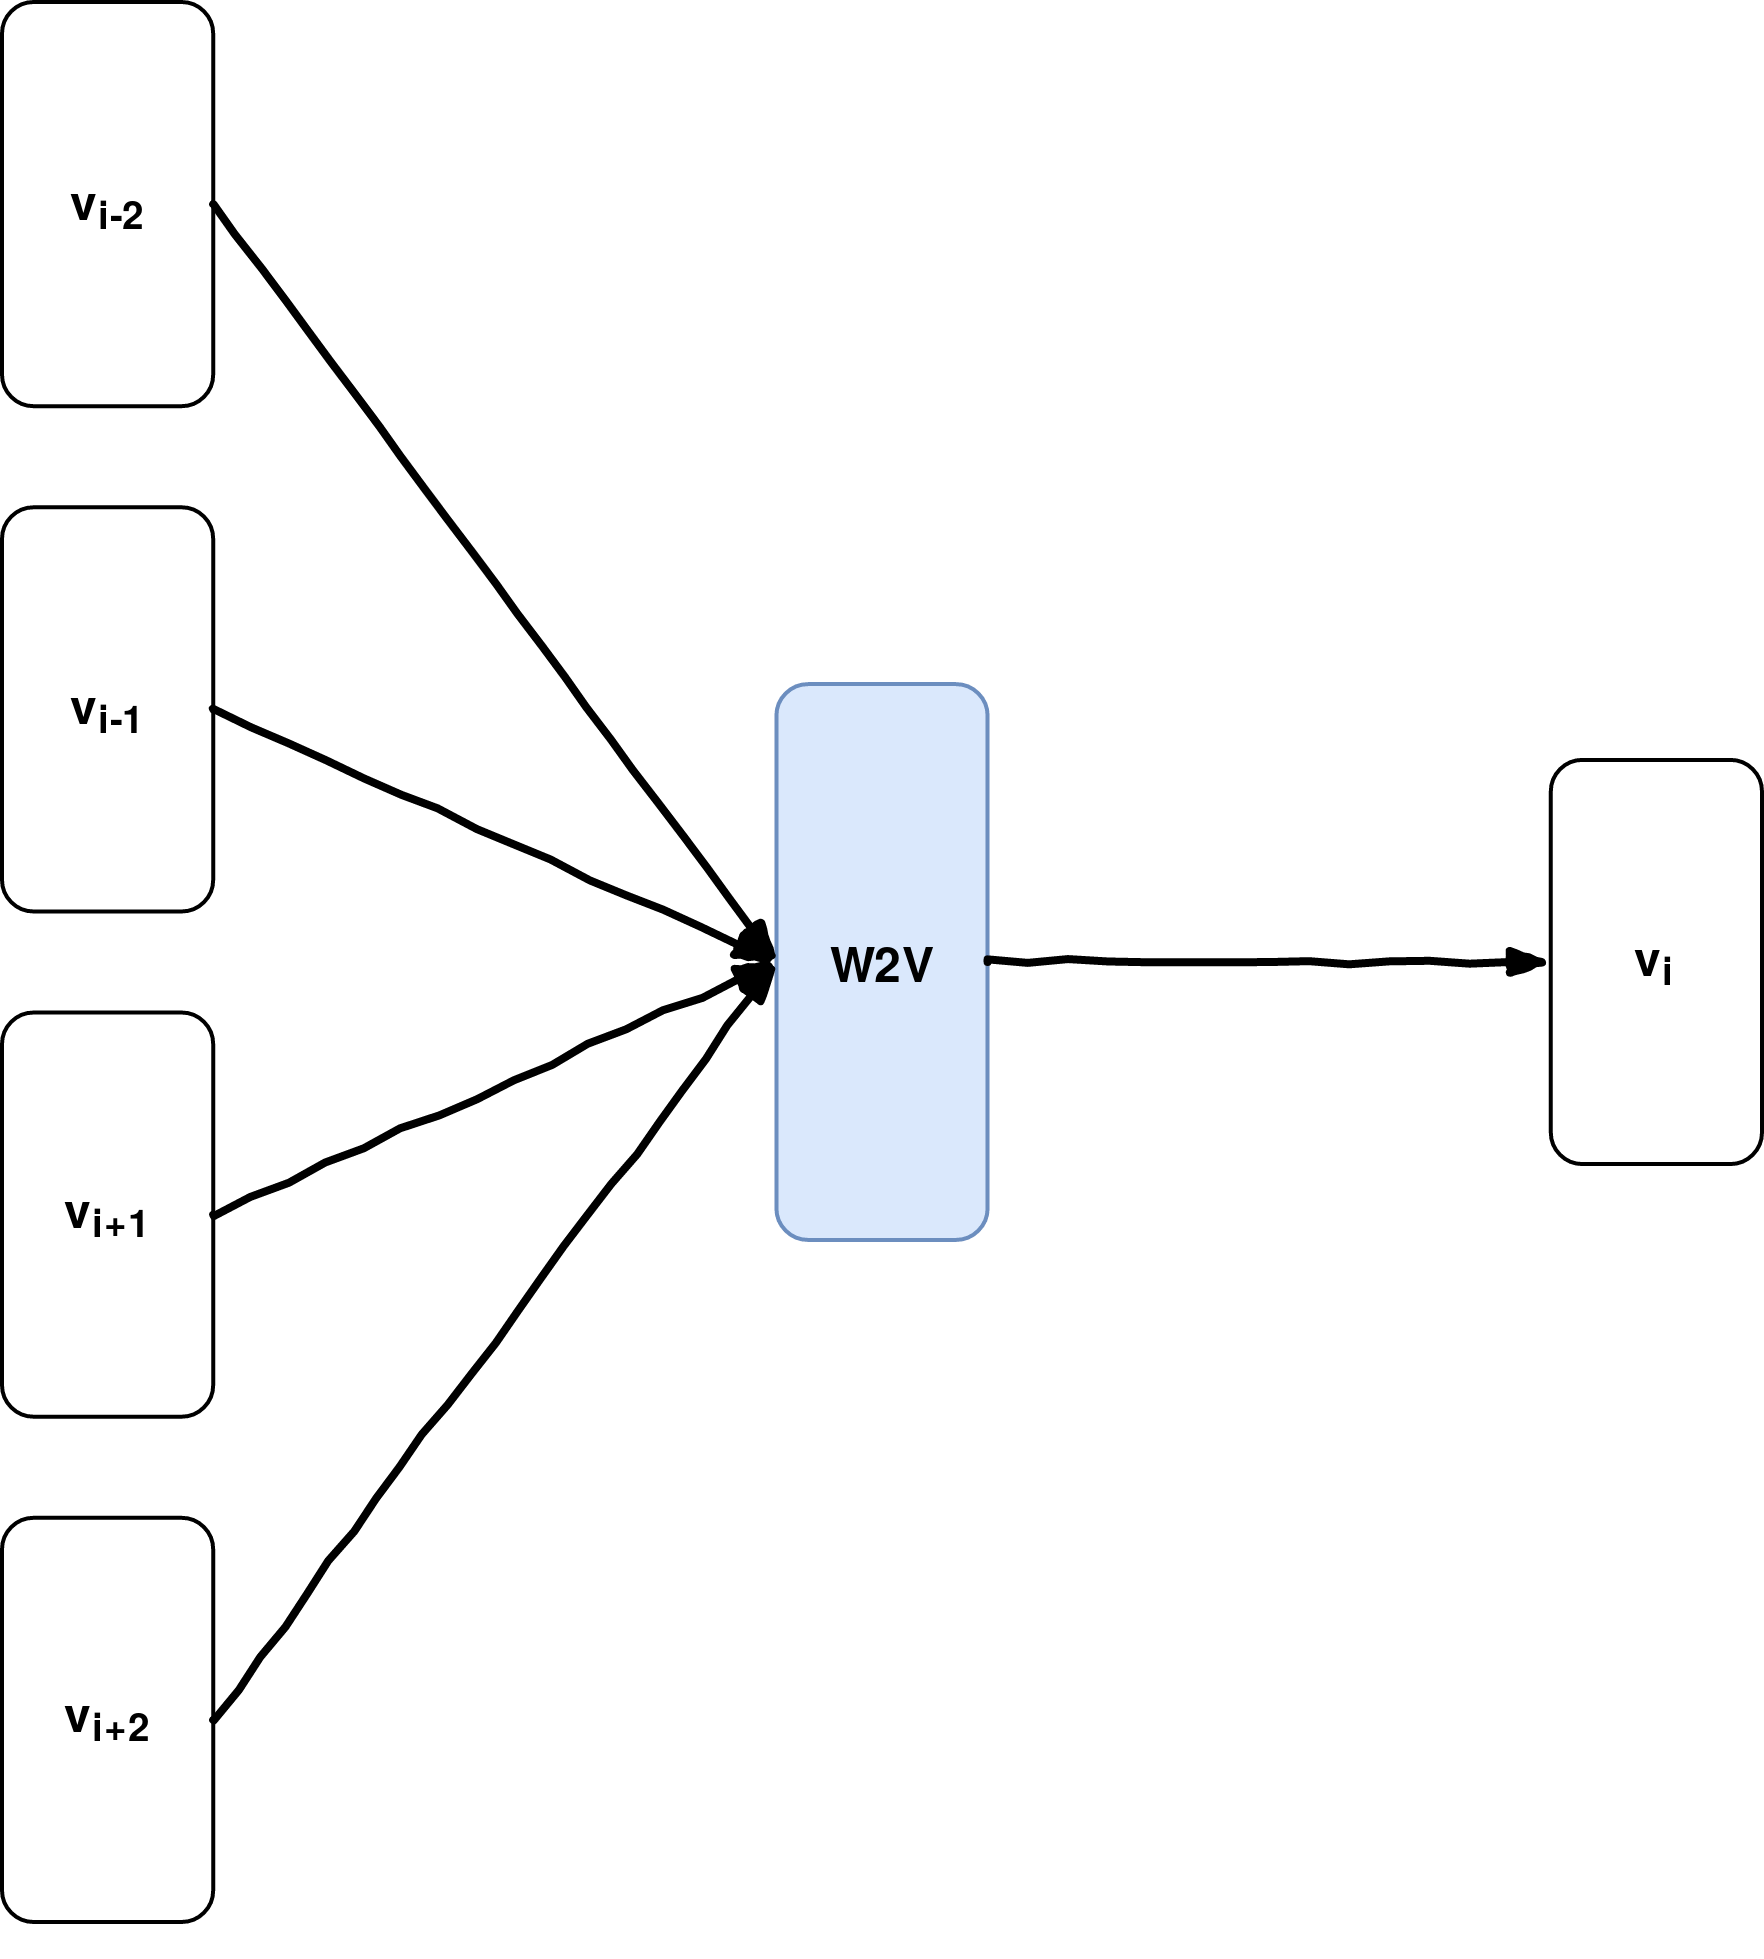
\includegraphics[width=0.5\textwidth,height=150px]{cbow}
	\caption{CBOW modell}
\end{figure}

Skip-Gram modell esetén pont az ellenkezője történik. A háló bemenete $v_i$
$\left( i \in \left|D\right| \right)$ vektor lesz. A tanítás célja, hogy a háló prediktálja az i. szó k méretű kontextusának one-hot kódolt vektorait ($v_{i-k},...,v_{i-1}, v_{i+1},..., v_{i+k} : k \in \mathbb{N}$), közben a háló a rejtett rétegében megtanulja a Word2Vec reprezentációt.

\begin{figure}[H]
	\centering
	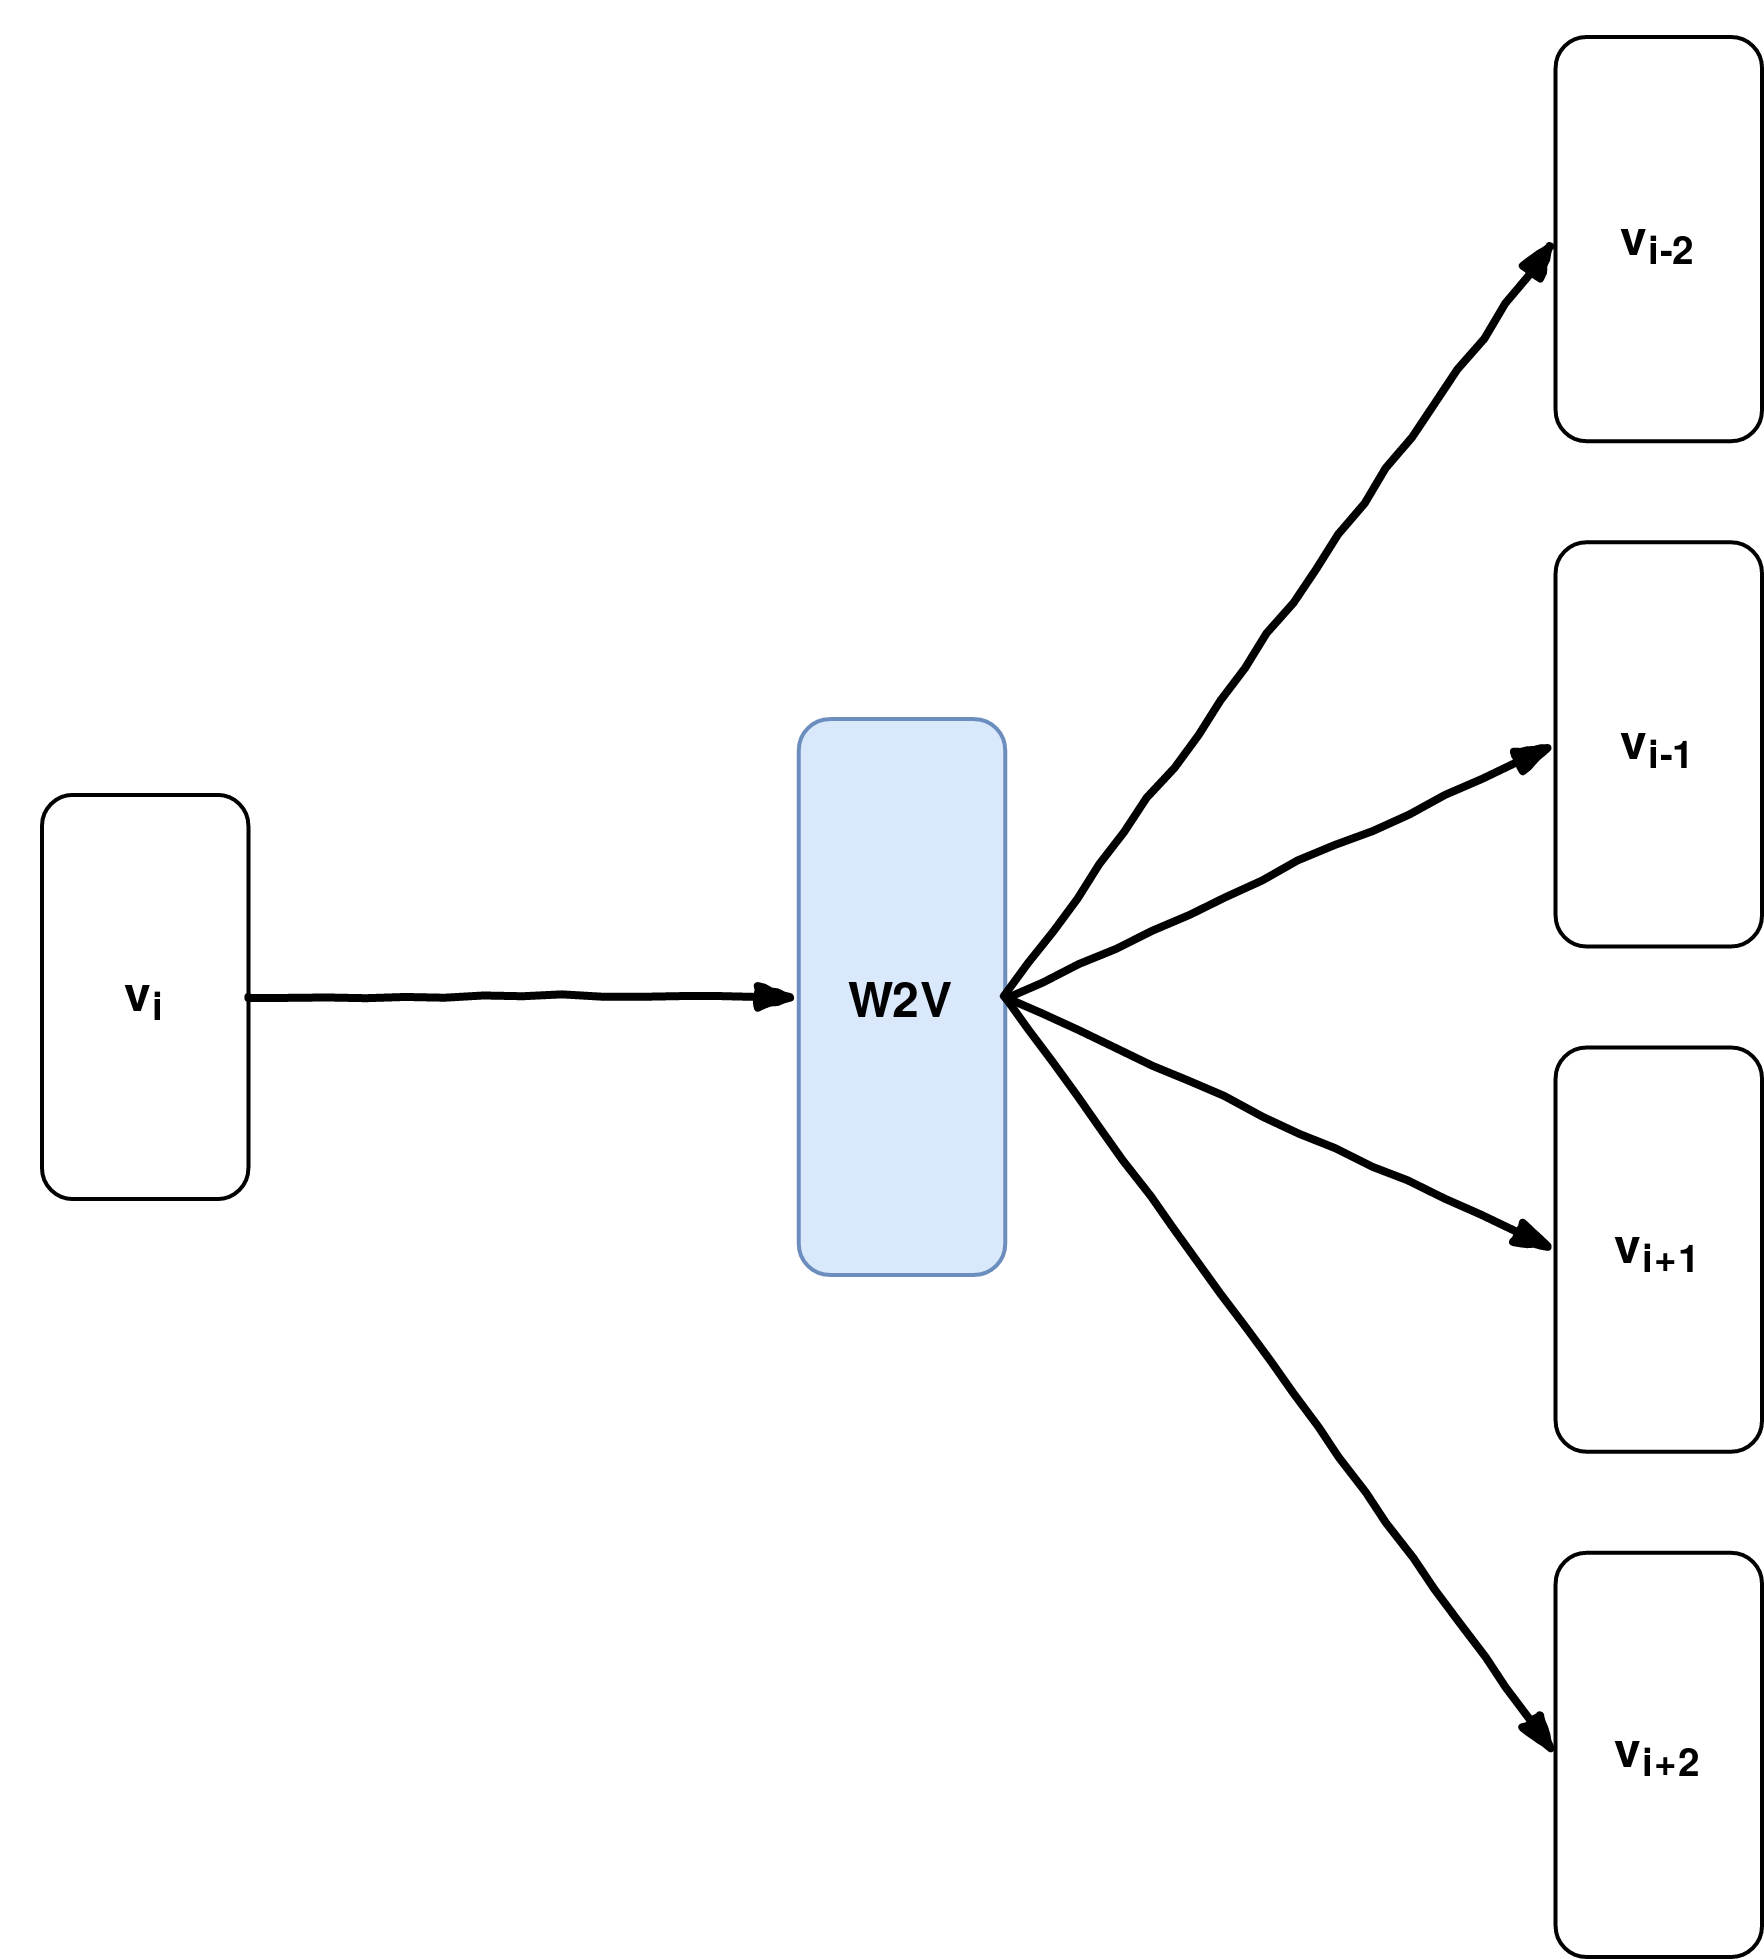
\includegraphics[width=0.5\textwidth,height=150px]{skip-gram}
	\caption{Skip-Gram modell}
\end{figure}

Egy jól tanított Word2Vec modell a hasonló jelentéstartalmú szóvektorokat közel re képezi egymáshoz a vektortérben. 
A teljesítmény növelése érdekében finomhangolhatjuk a tanítási paramétereket. Ilyen beavatkozás lehet ha növeljük a halmaz méretét, amellyel Word2Vec modellünket tanítjuk, vagy emeljük a kontextus ablak méretét és a reprezentációs dimenziót.

\begin{note}
	A Skip-Gram modell a ritka szavak, míg a CBOW modell a gyakori szavak esetén készít pontosabb reprezentációt.
\end{note}


\subsubsection{GloVe}
A Word2Vec bemutatását követő évben újabb nagy lépés történt a szóbeágyazás világában, a \textit{Stanford University} NLP kutatócsoportja publikálta a GloVe módszert.

A GloVe (\textit{Global Vectors}) \cite{pennington2014glove} reprezentációs módszer a Word2Vec-hez képest egy korpusz lokális statisztkáján kívül a globális statisztikáit is figyelembe veszi. 

\begin{definition}
	Adott egy korpusz, melynek elemszáma V. Az $X \in \mathbb{N}^{V \times V}$ mátrixot közös előfordulási mátrixnak nevezzük, ahol $X_{ij}$ az a szám, ahányszor i. szó kontextusában j. szó megjelenik.  
\end{definition}

A GloVe modell tanítása egy korpusz közös előfordulási mátrixának nemnulla elemein történik. A GloVe modell egy log-bilineáris modell, amely feladata, hogy kiszámítsa a következő szó valószínűségét azon kontextusa alapján.

A módszer mögötti intuíció az, hogy a közös előfordulási valószínűségek hányadosa értékes információval szolgálhat a leképezés során. Így a feladat célja, hogy a tanult szóvektorok skaláris szorzata megegyezzen a szavak közös előfordulási valószínűségének logaritmusával. Mivel $\log \left( \frac{A}{B} \right) = \log \left( A \right) - \log \left( B \right)$, így ez a cél összekapcsolja az előfordulási valószínűségek arányszámát a vektorok távolságával.

Ugyan a globális statisztikáknak köszönhetően a GloVe több feladatban is túlteljesíti a Word2Vec-et, a tanításához szükséges közös előfordulási mátrix memóriaigénye magas. Paraméterhangolás esetén újból fel kell építenie a mátrixot, mely költséges művelet.

\subsubsection{ELMo}
A Word2Vec és a GloVe már képes szemantikus információ leképezésére, azonban esetükben az ellentétes szópárok közel kerülnek egymáshoz. Azon feladatoknál, melyeknél az ellentétes szavak kiemelt szerepűek – például a hangulatelemzés – limitációk jelentkezhetnek, továbbá ezen algoritmusok rosszul kezelik az ismeretlen szavakat is.

Míg a Word2Vec és a GloVe csak szavankénti kontextusfüggetlen reprezentáció tanulására képes – azaz nem számít az adott szó környezete, melyre alkalmazzák –, addig az Embeddings from Language Models (ELMo) \cite{elmo} figyelembe veszi a lexémák kontextusát, mondaton belüli elhelyezkedését is. Az ELMo használat közben állítja elő a vektorokat.

A modell tanításához használt neurális háló több réteg kétirányú LSTM (biLSTM) konkatenációja. A különböző rétegek más és más típusú információt képesek eltárolni.

\begin{figure}[H]
	\centering
	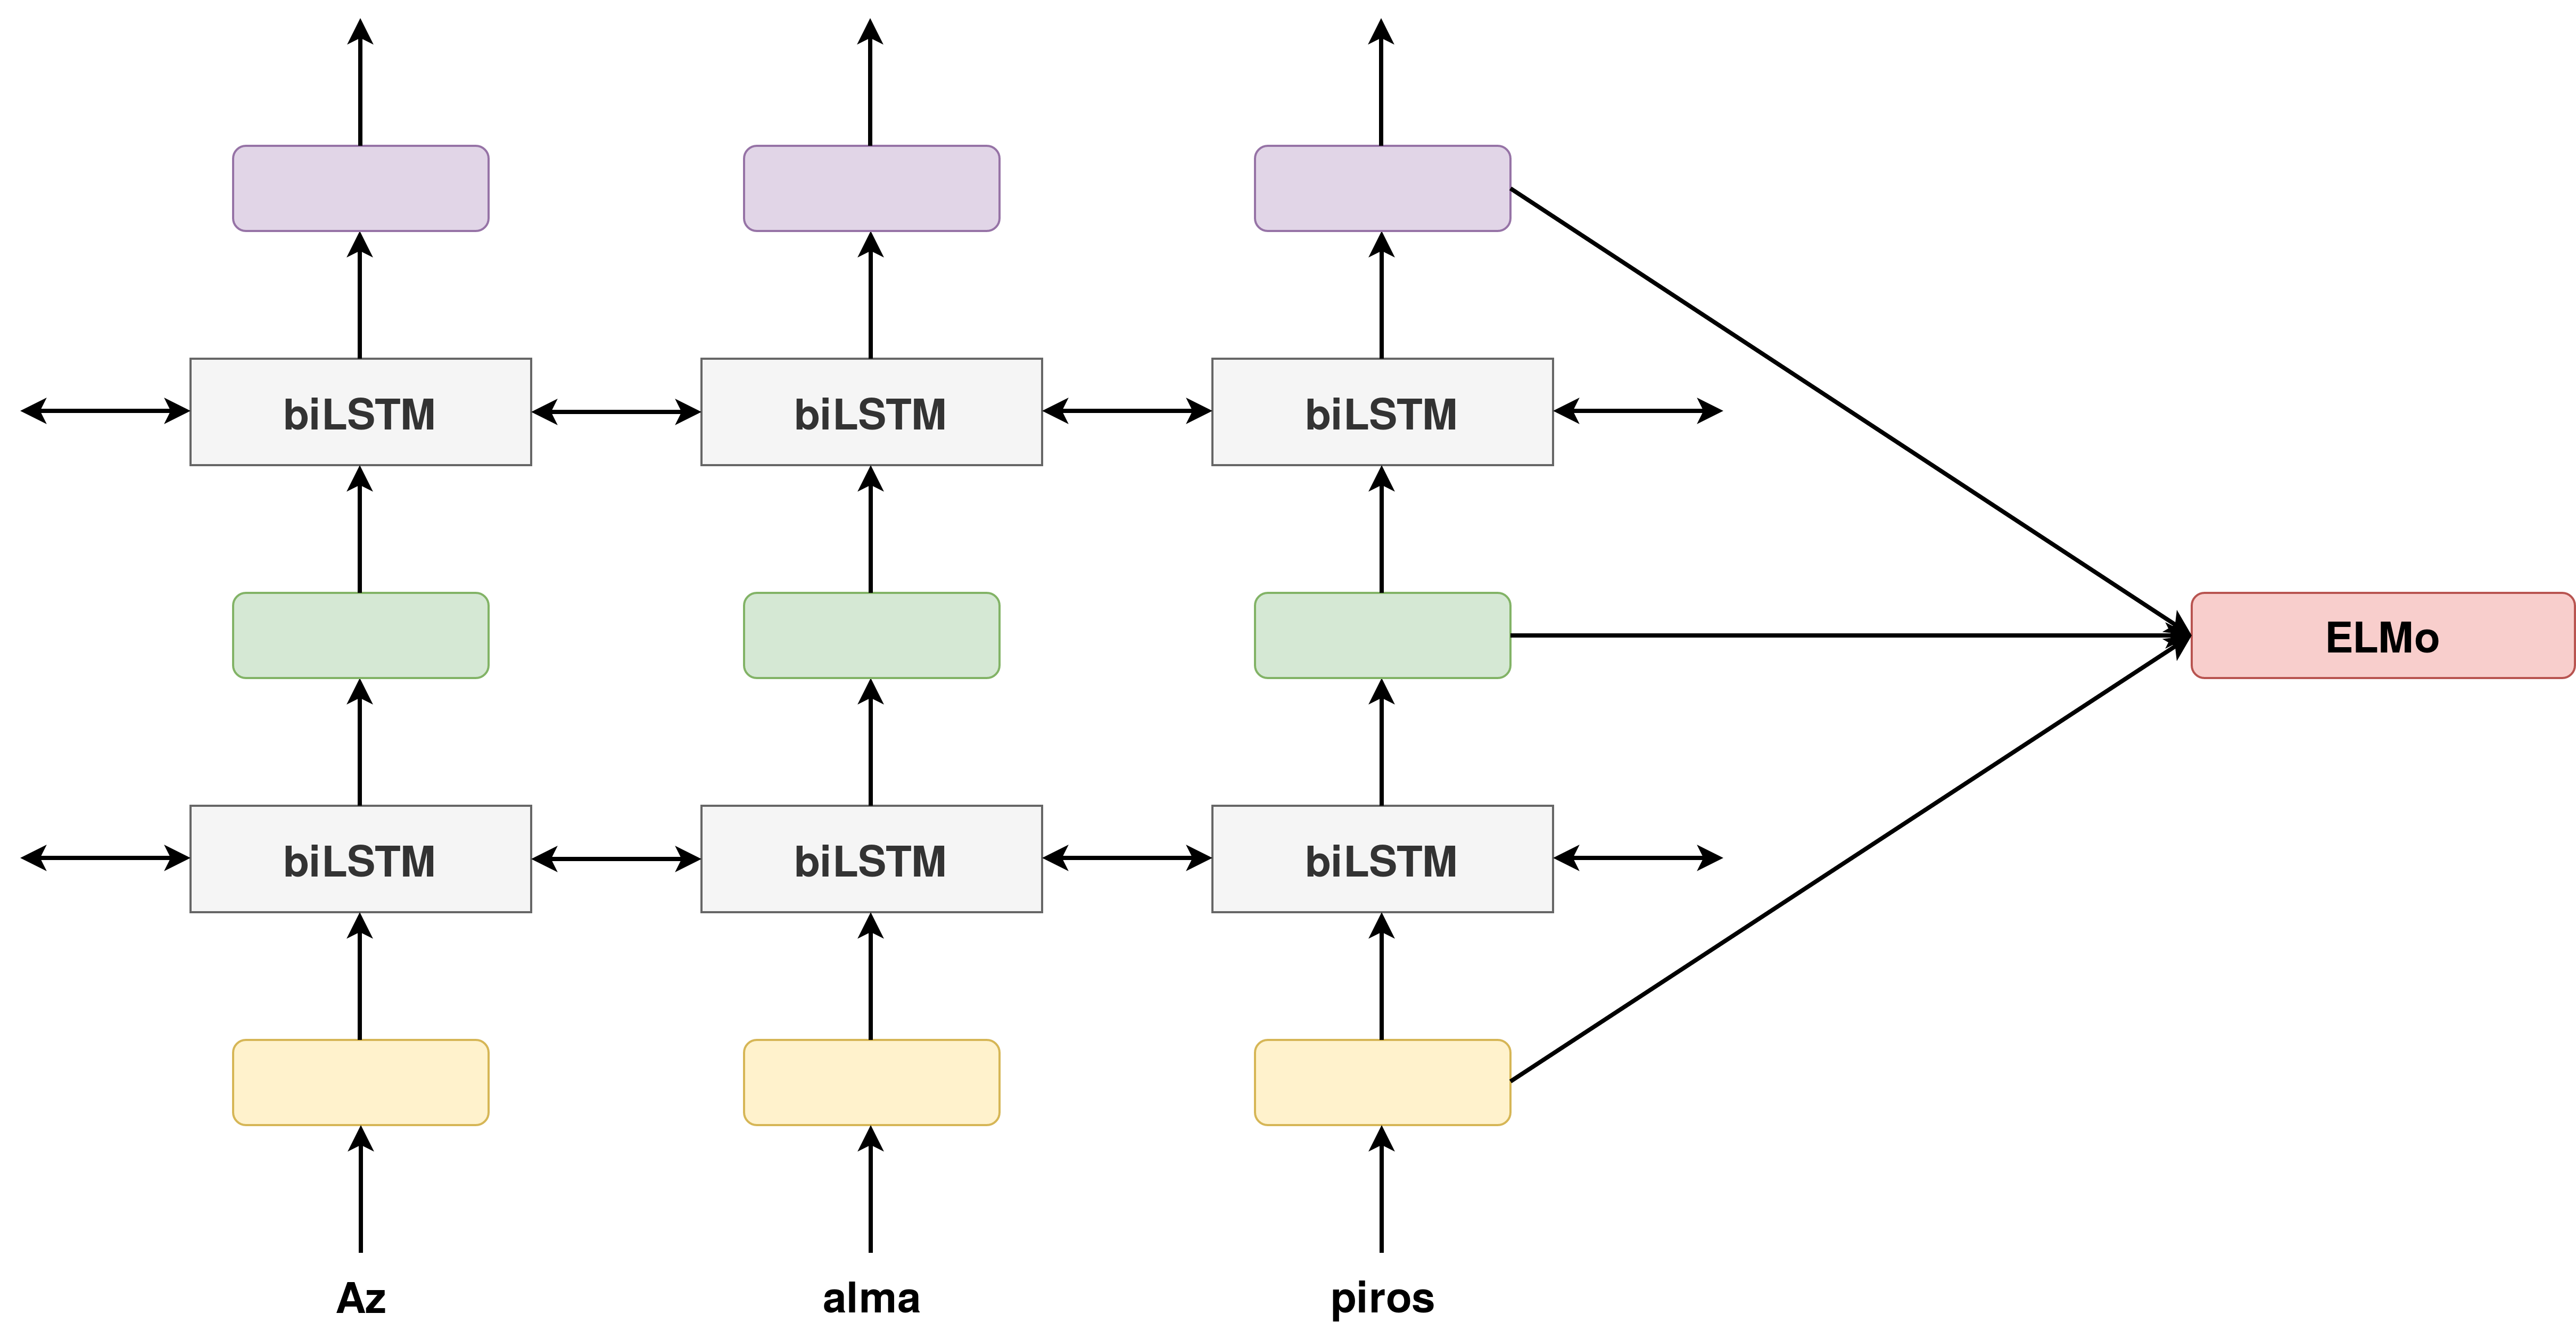
\includegraphics[width=0.8\textwidth,height=200px]{ELMo}
	\caption{ELMo modell}
\end{figure}

Az ELMo a különböző rétegek kimenetének feladatspecifikus kombinációján alapszik. Egy adott NLP feladatra minden BiLSTM réteg egyedi súlyt kap. A végső háló 2 darab BiLSTM rétegből áll, minden LSTM réteg 4096 széles.

Az így kapott sekély kétirányú módszer jelentősen javított a szóvektorok pontosságán.

Bár az ELMo egy karakter (konkatenáció) alapú reprezentációs algoritmus, szavakat ábrázol. Ezen tulajdonsága alapján képes kezelni az addig nem látott szavak problémáját is.


\subsubsection{BERT}
Egy 2018-ban publikált cikk \cite{char} rámutatott arra, hogy a karakteralapú algoritmusok nem teljesítenek olyan jól, mint a szóalapú társaik. A Bidirectional Encoder Representations from Transformers (BERT) \cite{2018arXiv181004805D} egy a Google által kifejlesztett transformer architektúrájú nyelvi modell. Az ELMo-hoz hasonlóan ez is kétirányú, azaz egy szó mindkét oldali kontextusát figyelembe veszi a tanulás alatt. A BERT azonban bemenetként nem szavakat és nem is karaktereket kap, hanem szótöredékeket.

A tanítást a \textit{transfer learning} szerint két fázisra bontották: előtanítás és finomhangolás. 

Az előtanítás két feladatból állt: \textit{következő mondat} és \textit{maszkolás}.
A bemenetben megadták a szótöredék token-eket, a token-ekhez tartozó mondaton belüli helyadatokat és azt, hogy az adott token A vagy B mondat közül melyikhez tartozik.

\begin{figure}[H]
	\centering
	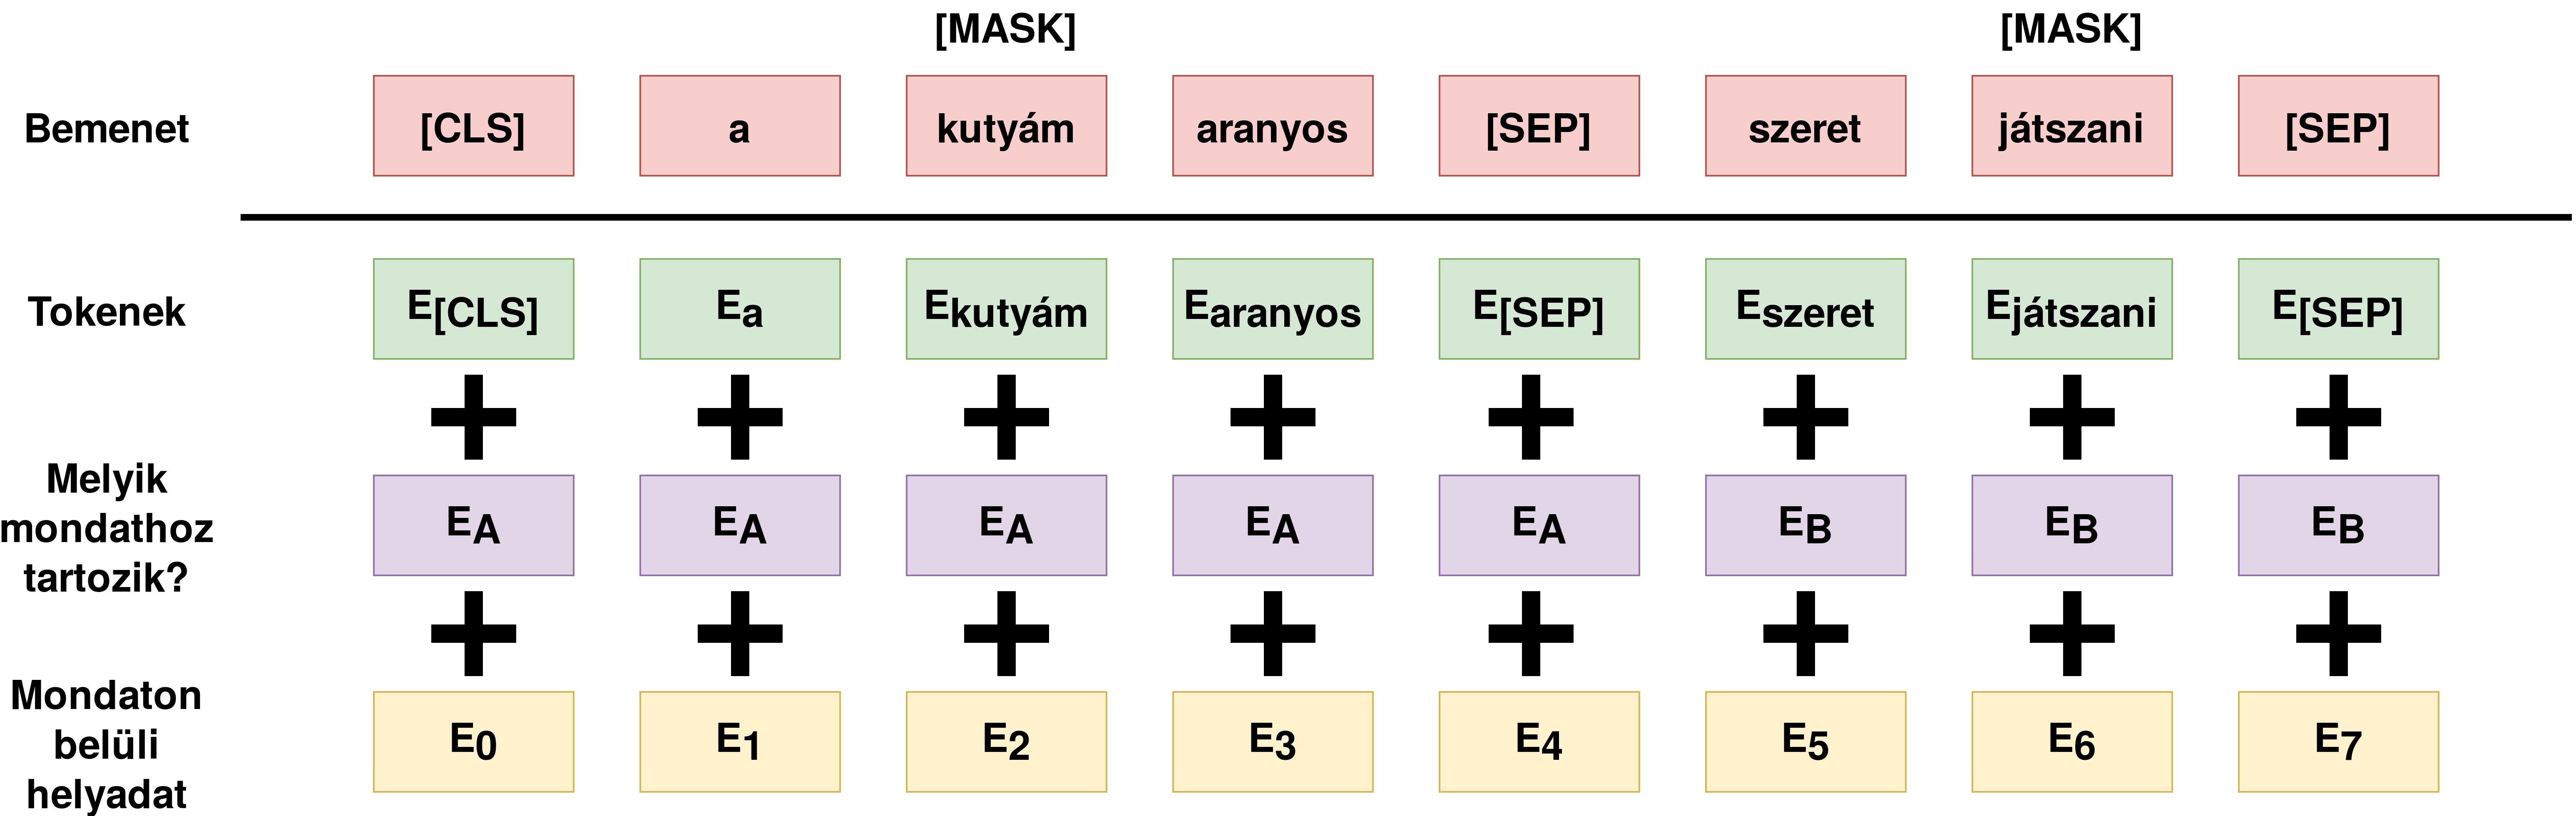
\includegraphics[width=1\textwidth,height=180px]{BERT}
	\caption{A BERT bemenete}
\end{figure}

 A \textit{következő mondat} esetében a mélyháló feladata kitalálni, hogy A[SEP]B input mondatokra B rákövetkezője-e A-nak. A \textit{maszkolás} során véletlenszerűen letakarták a token-eket a mondatokban és a mélyháló megpróbálta kitalálni, hogy eredetileg melyik szó volt a [MASK] token helyén.  A [CLS] token a klasszifikációs feladat alatt a mondatot ábrázolja, a [SEP] a mondatok közötti szeparátor és a [MASK] a letakart szótöredékeket helyettesíti.

A továbbiakban a modell finomhangolása az adott NLP feladat szerint történik.

Míg az ELMo különböző balról-jobbra és jobbról-balra olvasó rétegek konkatenációjaként állítja elő a vektorokat, addig a BERT a valódi mély architektúrájával csak egyszer dolgozza fel a token-eket. A \textit{transformer} architektúra nem igényel vektoriális bemenetet, saját reprezentációt épít a token-ek számára is.

A BERT szótöredék alapú megoldása egyesíti a karakteralapú modellek előnyét a szóalapú modellek előnyével. Képes kezelni az ismeretlen szavakat és performanciája mégis magas marad. A \textit{következő mondat} feladat a szövegben található mondatok közötti relációk, a \textit{maszkolás} pedig a mondatokon belüli szemantikai és szintaktikai információ ábrázolását segíti. Több NLP feladat megoldásában is jelenleg a BERT a \textit{State-of-the-art}.

\section{Reprezentáció a mondatok és magasabb nyelvi elemek szintjén}

Ahogy a lexémák szemantikai tartalmát sem határozza meg az őket alkotó karakterek lánca, úgy a mondatok sem értelmezhetőek pusztán a magukban foglalt szavak halmaza alapján. A mondatok és magasabb nyelvi elemek interpretálása során fontos tényezők lehetnek a bennük lévő szintaktikai viszonyok és a kontextus is.

Néhány NLP feladatnál, mint például a dokumentumok szemantikus keresésénél, vagy szöveg összegzésnél szükség lehet magasabb szintű reprezentációkra.  Ezek a módszerek szavak helyett mondatokat, bekezdéseket, vagy akár egész dokumentumokat tesznek numerikusan értelmezhetővé. 

\subsection{Mondatvektorok}
A szóvektorokhoz hasonlóan úgy kaphatunk mondatvektorokat, ha mondatokat helyezünk el egy vektortérbe. A tanítás során azonban a sorrendiség, az egyes lexémák változó súlya és a szintaktikai viszonyok megnehezíthetik dolgunkat. Szükség van egy technikára, mely segítségével leképezhetjük és szemantikai tartalmuknál fogva összegezhetjük a megfelelő rendezett szóvektorok sorozatát, így hozzájutva az adott mondat reprezentációjához. A módszerünk akkor hatékony, ha az azonos jelentéstartalmú mondatvektorok klaszterekbe tömörülnek a vektortérben.

\subsubsection{Skip-thought vektorok}
A Skip-though \cite{skip} egy 2015-ben bemutatott mondatreprezentációs módszer – a Skip-Gram algoritmus kiterjesztése – , amely a környező mondatokat is figyelembe veszi a tanulás során. 

A szerzők rekurrens enkóder-dekóder architektúrát használtak a tanításhoz. A neurális háló bemenete mondathármasok szavainak Word2Vec vektoraiból állt. A háló feladata $s_i$ mondat esetén $s_{i-1}$ és $s_{i+1}$ mondatok generálása volt.

\begin{figure}[H]
	\centering
	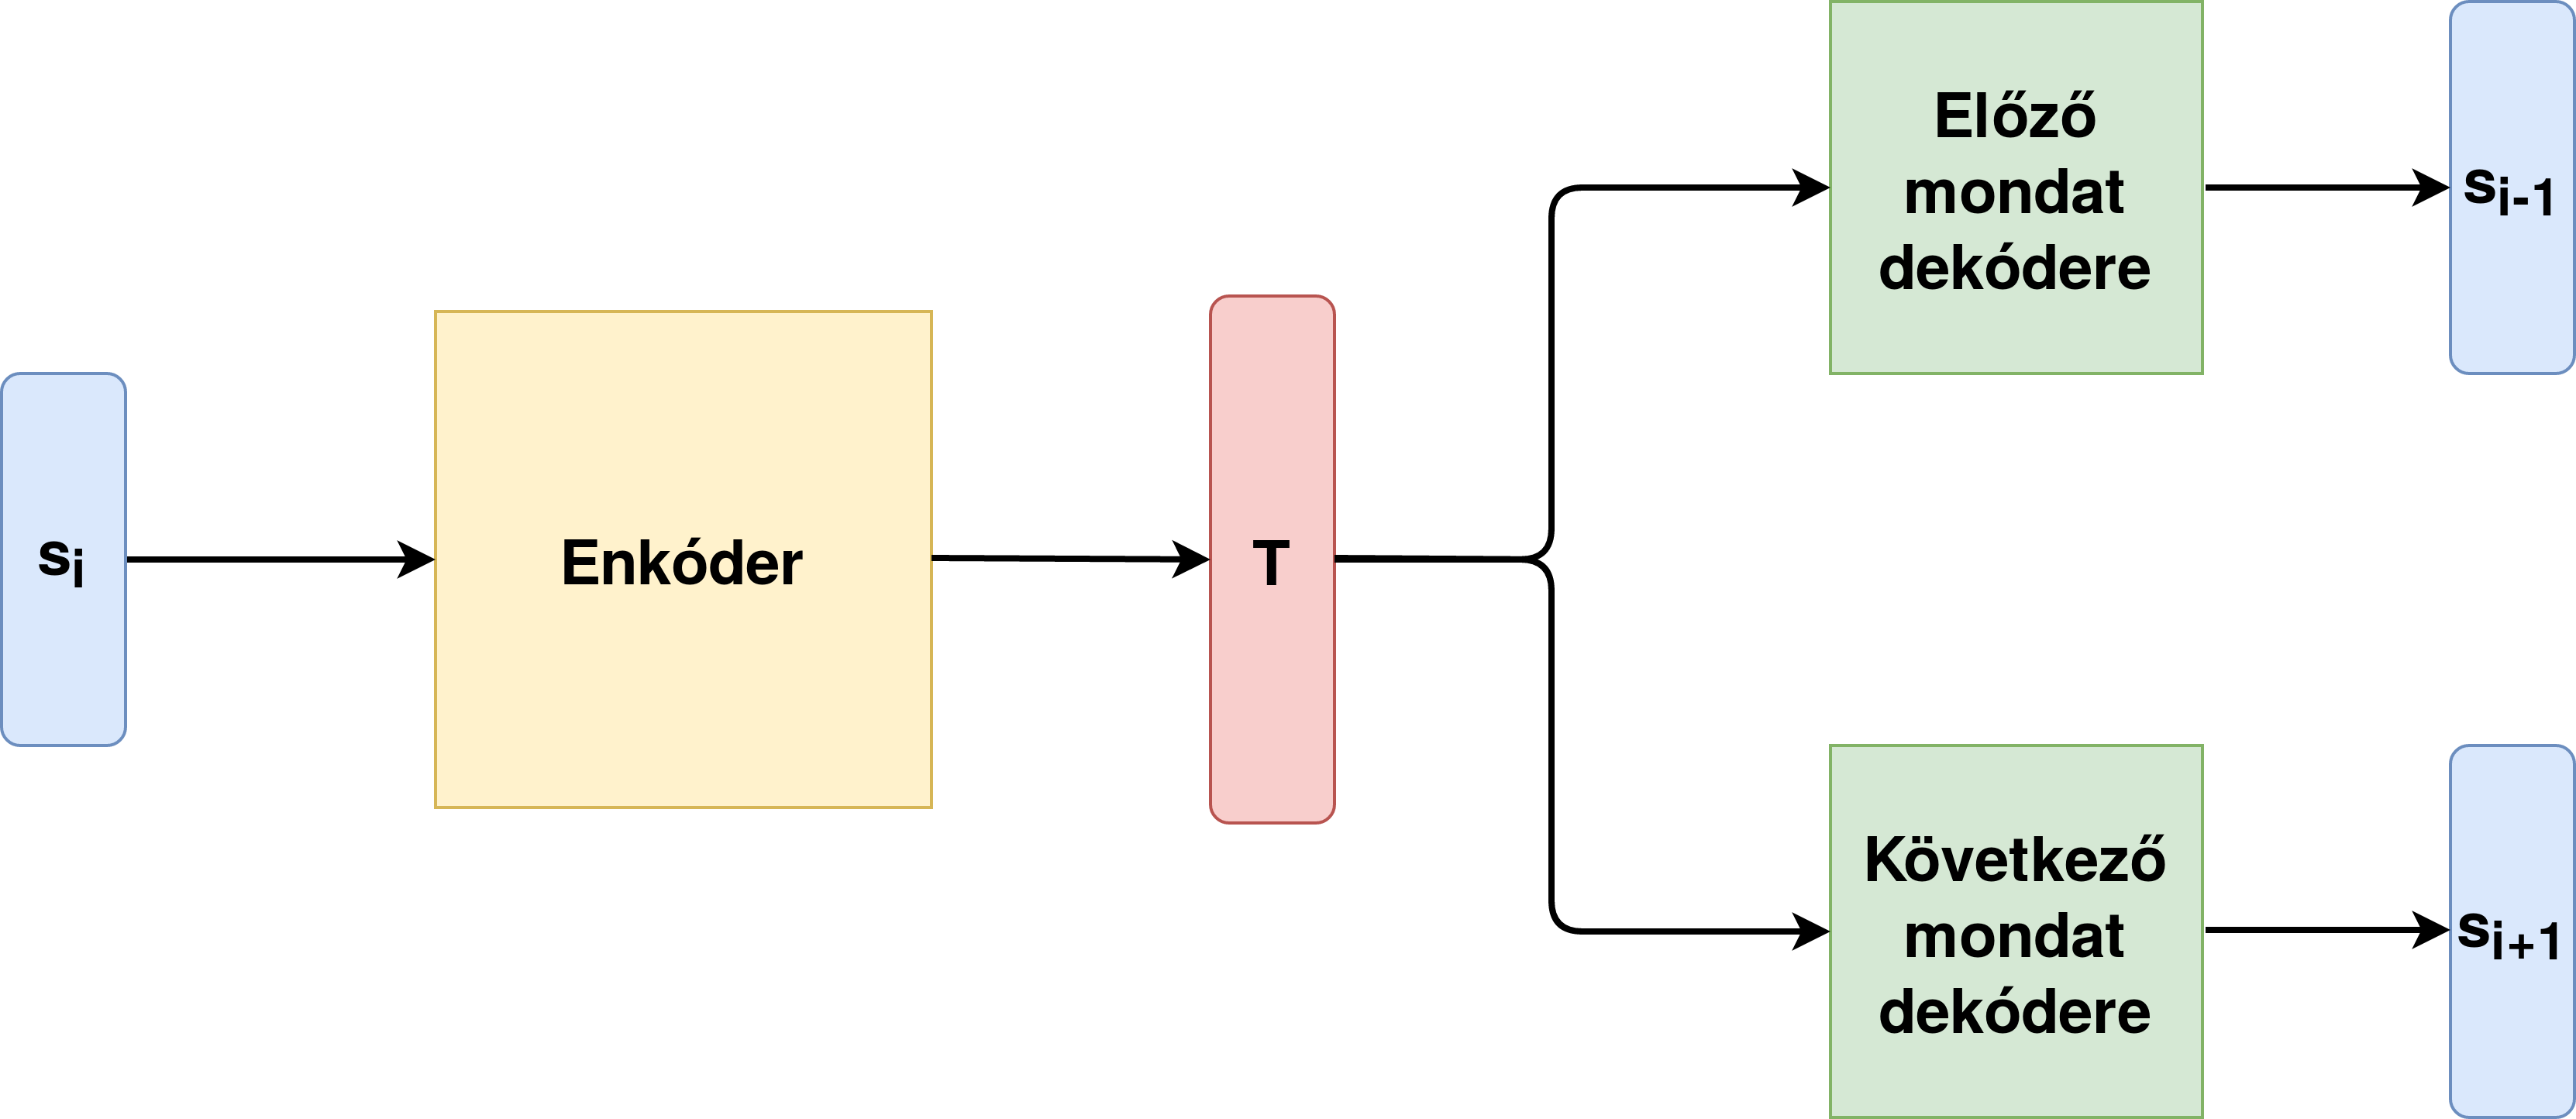
\includegraphics[width=0.6\textwidth,height=130px]{Skip-thought}
	\caption{A Skip-thought enkóder-dekóder architektúrája}
\end{figure}

Az enkóder és dekóder blokkokhoz rekurrens hálót használtak, melyek lehetnek LSTM és GRU rétegek is. Az enkóder célja a legjobb teljesítményével segíteni a dekóder blokkokat, míg a dekóder blokkok célja minimalizálni az előző és a következő mondat rekonstrukciós hibáját.


Olyan szavak esetén, melyeket a háló még nem ismert, tanítottak egy $f:V_{w2v} \rightarrow V_{rnn}$ lineáris leképezést, ahol $V_{w2v}$ és $V_{rnn}$ rendre a Word2Vec és a rekurrens modell szótára. A reprezentáció vektora a rejtett, úgy nevezett \textit{thought} vektor (T).

Bár a \textit{Skip-thought} módszer képes a mondaton belüli és kívüli sorrendiségi információ leképezésére is, csak olyan esetben teljesít megfelelően, ahol az egyes mondatok – melyekre alkalmazzák – megfelelő kontextusban szerepelnek, nem izoláltak.

\subsubsection{InferSent}
2017-ben a Facebook kutatói jelentős áttörést értek el a mondatszintű reprezentációs módszerek terén, a technika neve InferSent \cite{infer}. Hasonló algoritmusokkal ellentétben a szerzők felügyelt tanítást végeztek, melyhez az SNLI adathalmazt vették igénybe. A cikk megmutatta, hogy egy kisebb adathalmazon történő felügyelt tanítás felülmúlhatja a nagyobb adathalmazon nem felügyelt módon tanított modellek teljesítményét.

Az SNLI adathalmaz 570 ezer darab – ember által írt és címkézett – mondatpárból áll. A címkék a következők: következmény, ellentmondás és semleges.

Négyféle neurális architektúrát összemérve a legpontosabb eredményt a BiLSTM + max pooling mutatta. 

\begin{figure}[H]
	\centering
	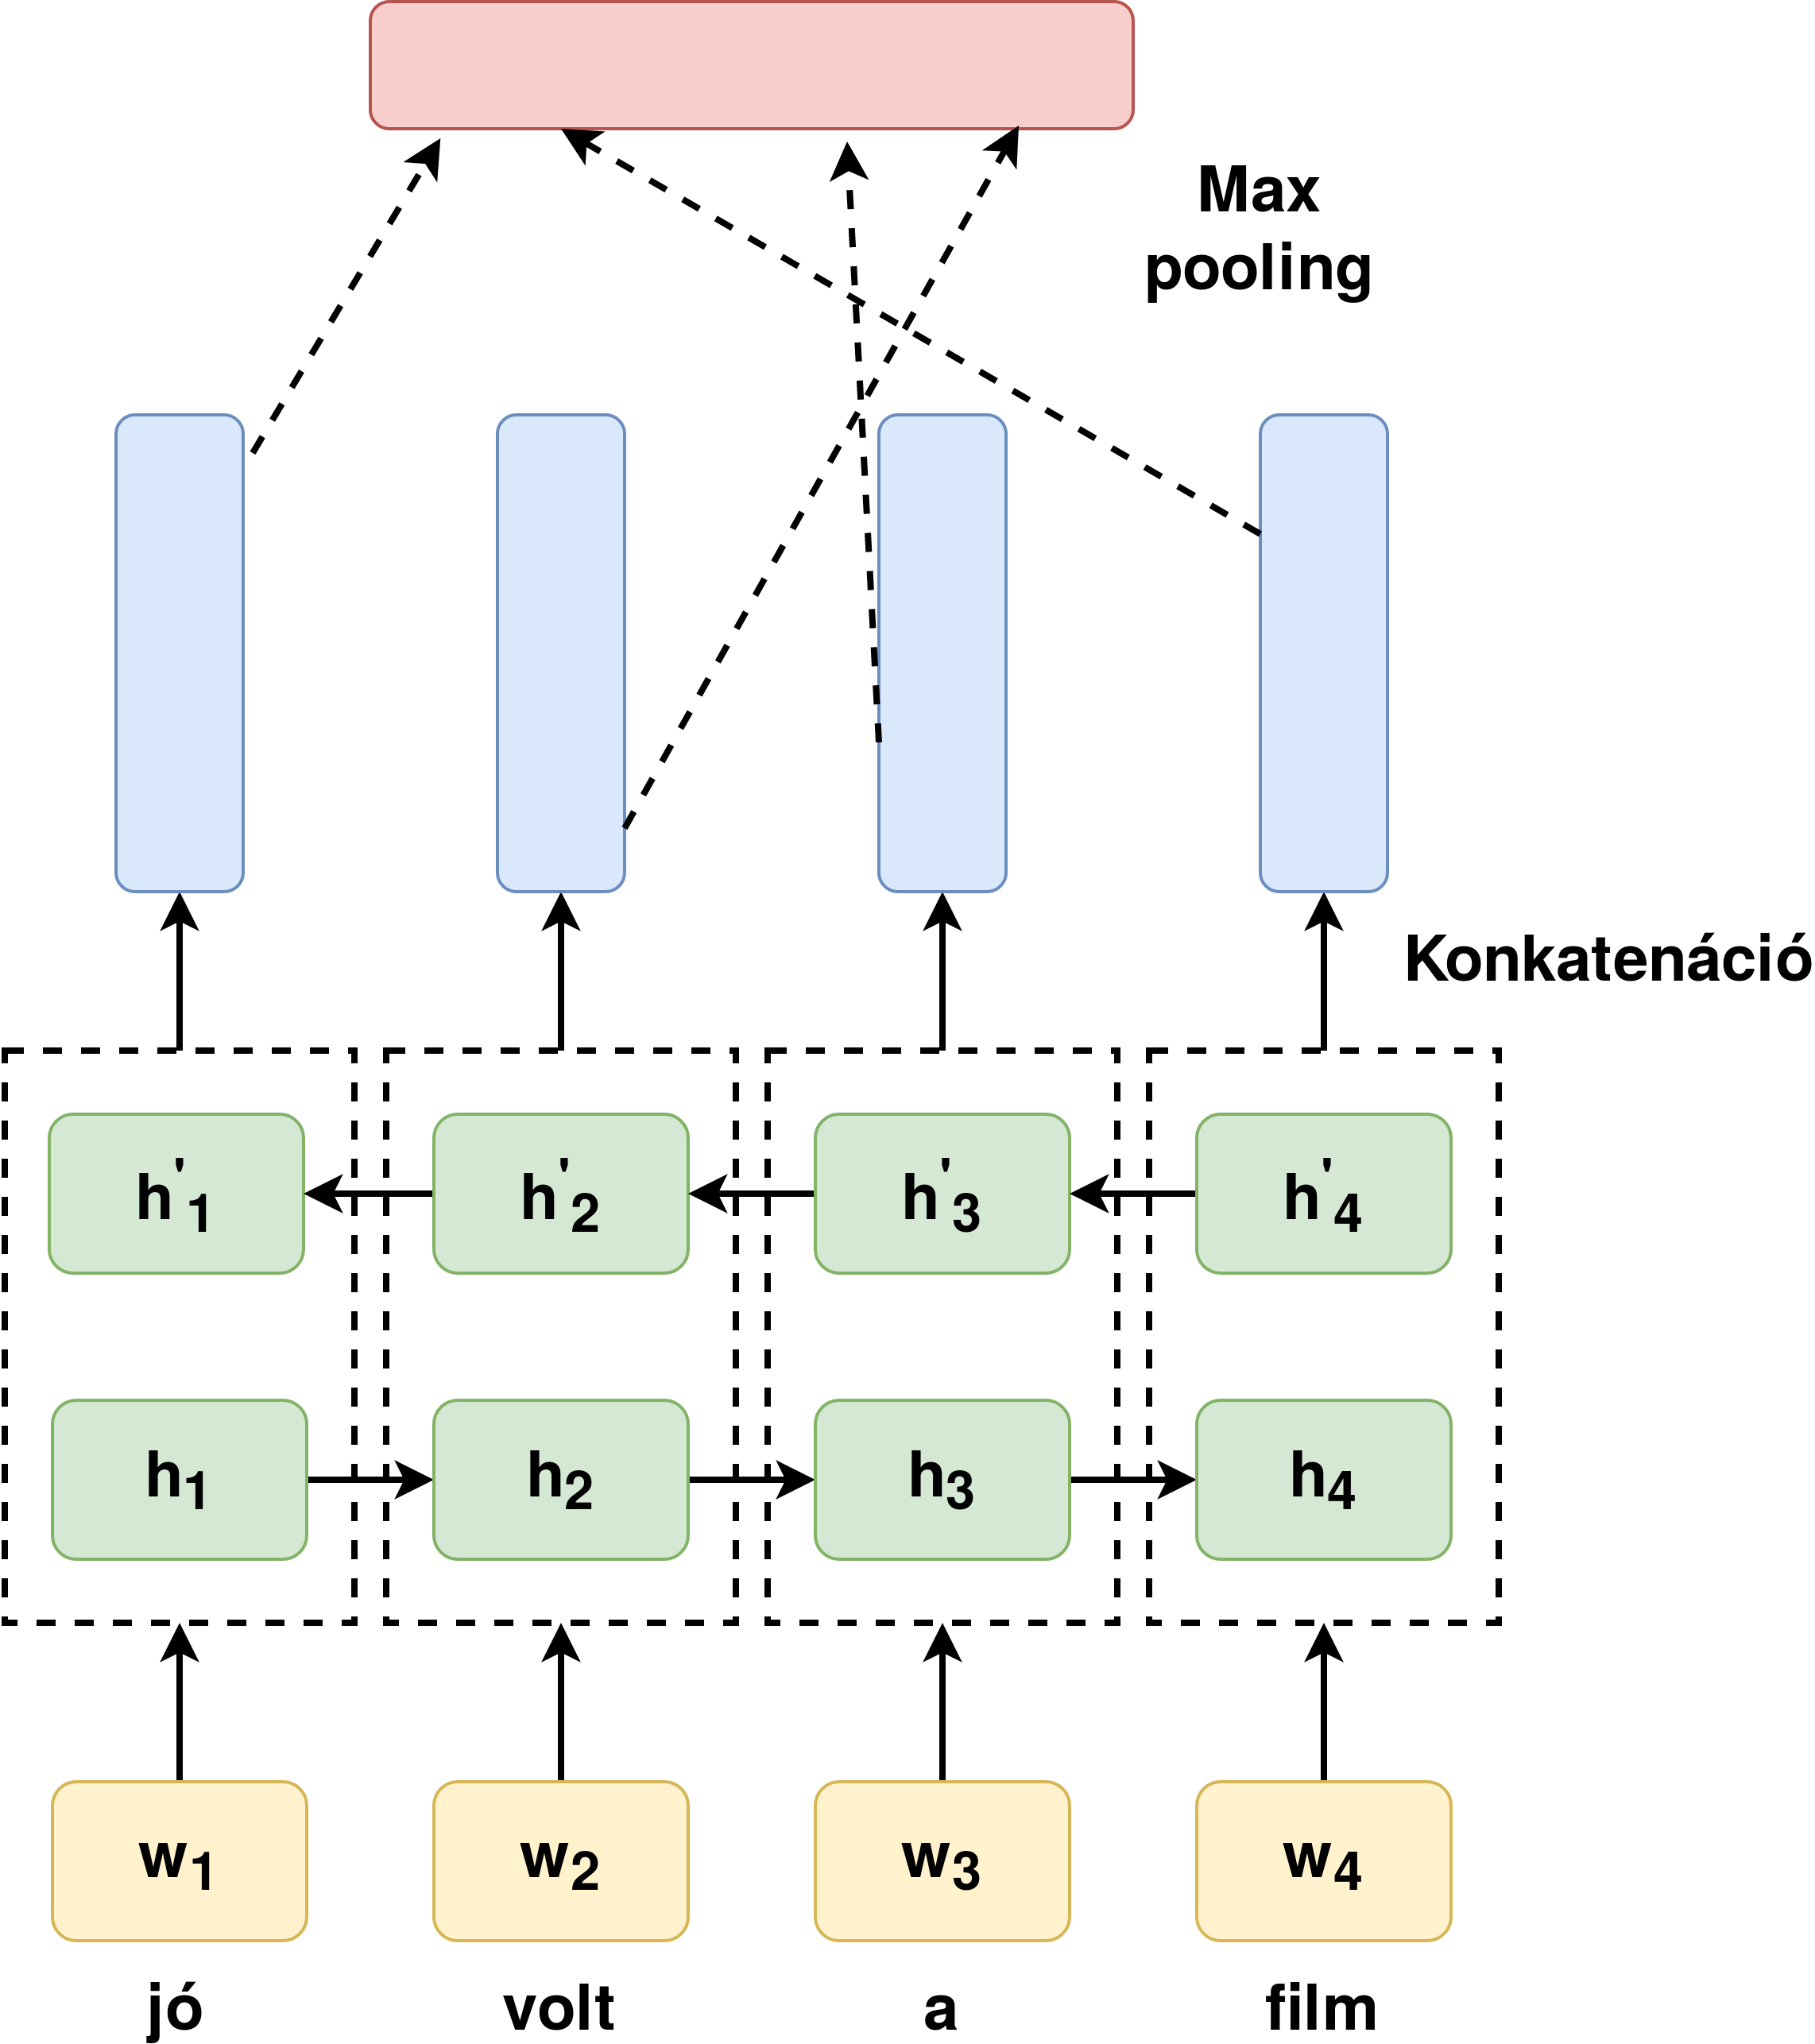
\includegraphics[width=0.5\textwidth,height=200px]{biLSTM-max-pooling}
	\caption{A BiLSTM + max pooling architektúra}
\end{figure}

Az SNLI feldolgozásához szükséges NLI feladat speciális szerkezetet igényel. Mivel kontextusfüggetlen reprezentációt akartak előállítani, amely izolált formában is működik, a mondatpárok GloVe vektorait szeparáltan enkódolták.

\begin{figure}[H]
	\centering
	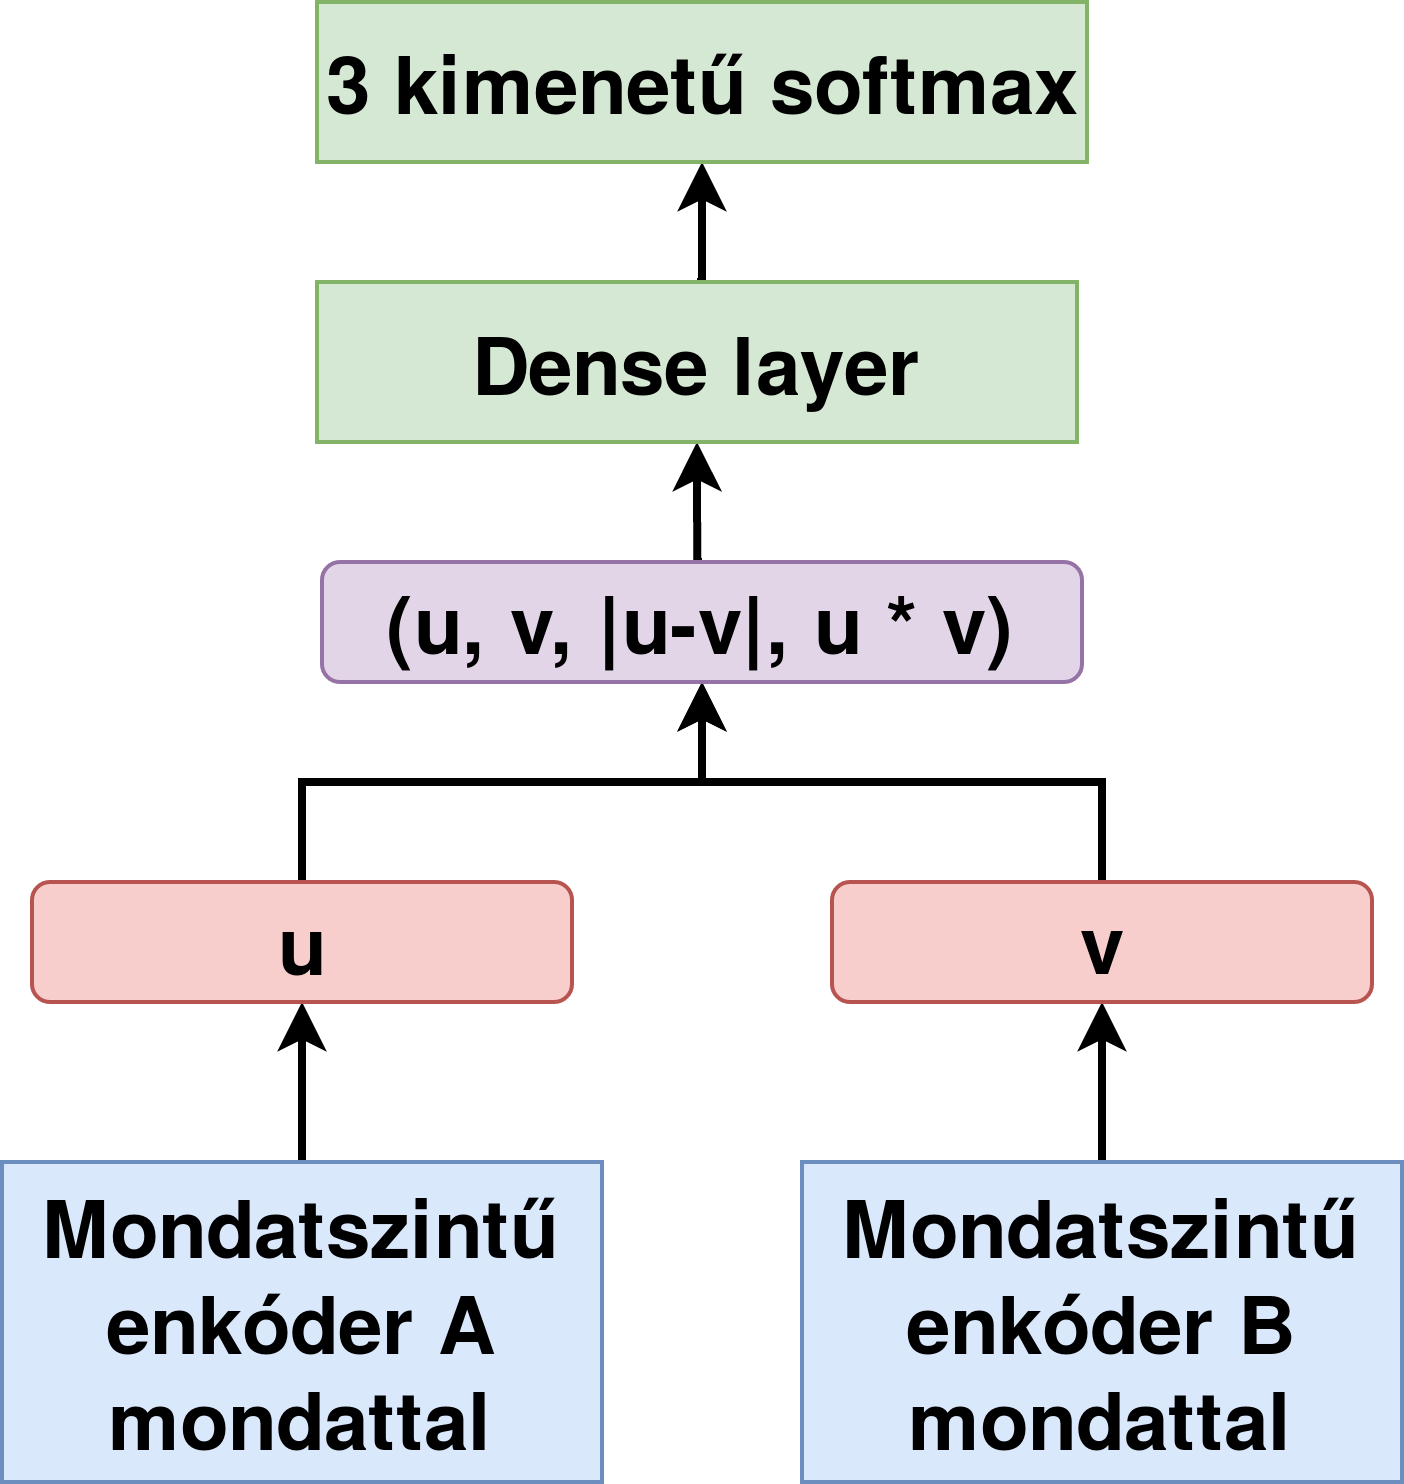
\includegraphics[width=0.5\textwidth,height=150px]{NLI}
	\caption{Az NLI feladat}
\end{figure}

Az így készült u és v vektorokból egy speciális reprezentáció készült: u, v, $\left| u - v \right|$ és $u \ast v$ (vektoriális szorzat) konkatenációjával, melyet végül egy 3 osztályú klasszifikáló hálóba vezettek.

A szerzők a reprezentációs vektorméret növelésével pontosabb eredményt kaptak, de a vektorok memóriaigénye emelkedett. Az InferSent megoldja a kontextusfüggőség problémáját, így a módszer már szövegrészletekre is alkalmazható.

\begin{note}
	Az InferSent napjaink egyik legjobb teljesítményű szemantikus reprezentációs algoritmusa.
\end{note}

\subsubsection{USE}
Az InferSent bemutatását követő évben a Google Research csapata a modern reprezentációs módszereket vizsgálta a \textit{transfer learning} aspektusából. A Universal Sentence Encoder (USE) \cite{use} egy mondatszintű  algoritmus, mely célja, hogy a használója könnyedén igényeire tudja formálni, annak érdekében, hogy pontosabb leképezést kapjon. A szerzők két architektúrát használtak: a BERT-ben említett \textit{transformer}-t és a DAN-t (\textit{Deep Averaging Network}). 

\begin{figure}[H]
	\centering
	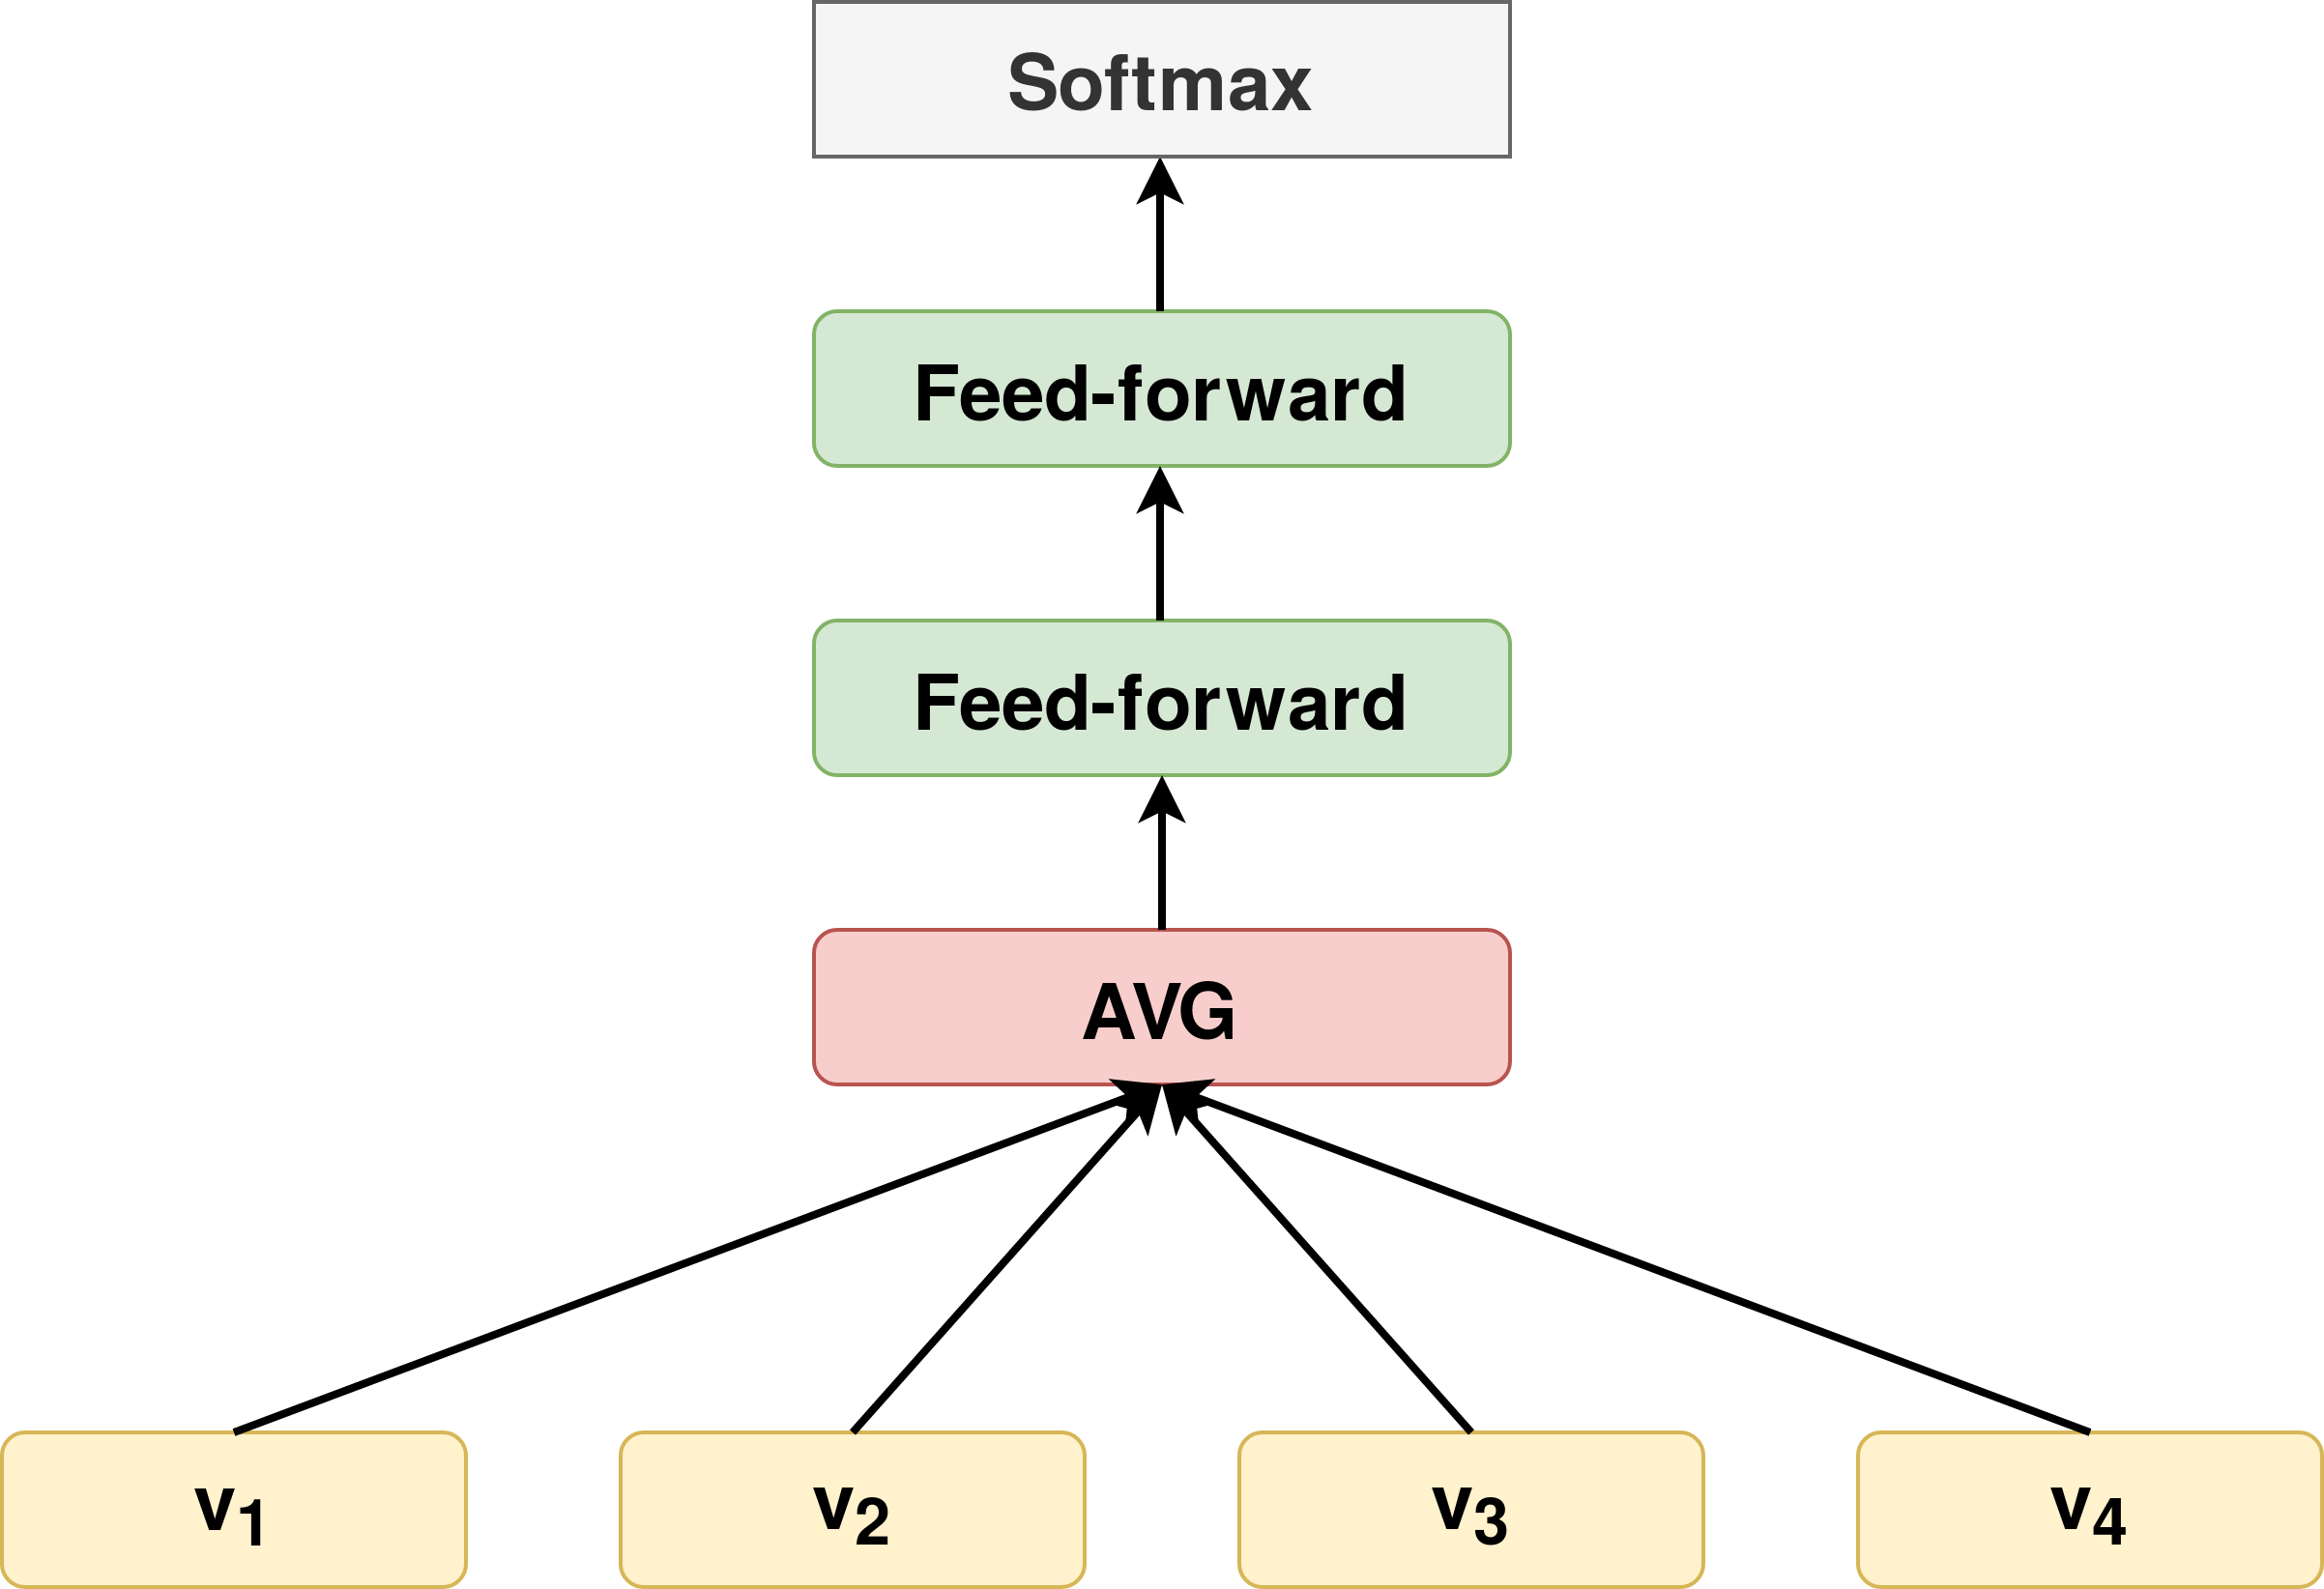
\includegraphics[width=0.6\textwidth,height=150px]{DAN}
	\caption{DAN architektúra}
\end{figure}

A \textit{transformer} modell egyik algráfja a mondatokban lévő szavak kontextusfüggő reprezentációját állítja elő. A folyamat során figyelembe veszi az egyes lexémák sorrendi és egyéni információit is, majd összegzi őket, így megkapja a végső mondatszintű reprezentációt.
A \textit{DAN} modell az input tokenek vektorait először átlagolja, majd \textit{feed forward} rétegek segítségével előállítja a mondatvektorokat. A USE szavakból, mondatokból, vagy akár rövidebb bekezdésekből is képes 512 méretű vektorokat generálni.

A neurális hálók tanítását két részre bontották, bemenetként angol nyelvű karakterláncokat kaptak. Az első rész a \textit{Skip-thought}-hoz hasonló módon, dialógusokból vett mondat-válasz párokkal, illetve felügyelt módon a \textit{Stanford Natural Language Inference} (SNLI) korpuszon történt.

A cikk során kiemelt szerepet kapott a tanítás második fázisa. Számos módon finomhangolták a modelleket és mérték a teljesítményüket. A feladatok közé tartozott, hogy filmes értékelések szövege alapján ki kellett találnia a neurális hálóknak az értékelések pontszámát 1 és 5 között. Továbbá vásárlói értékelések hangulati töltetét kellett prediktálniuk.

 Az algoritmusokat kipróbálták a szavak szintjén, a mondatok szintjén és a kettő módszer konkatenációjaként is. A legjobb teljesítményt a mondatszintű reprezentációk mutatták. A transformer architektúra pontosabb eredményt hozott, mint a DAN alapú modell, de a transformer modell $\mathcal{O}(n^2)$, míg a DAN modell $\mathcal{O}(n)$ időkomplexitású a bemeneti hossz függvényében. Továbbá memóriahasználatban is kedvezőbb választás a DAN.

A \textit{GloVe}-hoz hasonlóan a USE is képes asszociációkra, de jóval gyengébb ezen képessége az olyan kényes témák esetében, mint a szexizmus és a rasszizmus. Ez a tény alkalmassá teheti a USE-t az ipari használatra is.

A szerzők rávilágítottak arra, hogy kevés adat esetén jó választás lehet a \textit{transfer learning} módszere, és a magasabb szintű reprezentációk pontosabb eredményt érhetnek el a legtöbb feladat esetében.

\subsection{Dokumentumszintű reprezentáció}
Ahogy a technológia fejlődik, úgy növekszik a világon az egységnyi idő alatt előállított információ mennyisége is. Gyakori eset, hogy ez írott formában, dokumentumokban jelenik meg. Dokumentumnak tekinthetünk minden, a mondatnál hosszabb emberi nyelven írott szöveget.

Bár a magasabb nyelvi egységek értelmezése és feldolgozása sok területen előkerülő feladat, mégsem triviális. Nagy kihívást jelent a szemantikai szimilaritás mérése, az olyan gyakorlati problémákat nem is említve, mint a duplikációk kiszűrése a fórumokról, vagy a szociális média analízis.

2014-ben a Word2Vec szerzői előálltak egy dokumentumszintű reprezentációs algoritmussal. A Doc2Vec \cite{le2014distributed} módszer a Word2Vec modell kiterjesztése a dokumentumok szintjére. Mivel a dokumentumokat nem lehet a szavakhoz hasonló logikai struktúrába rendezni, ezért a megszokott \textit{CBOW} modell bemeneti vektorai mellé egy speciális, a magasabb nyelvi elem azonosítóját jelölő vektort konkatenáltak. Az algoritmus neve PV-DM. A modell tanítása végén a speciális vektor reprezentációja képviseli a dokumentumot.

\begin{figure}[H]
	\centering
	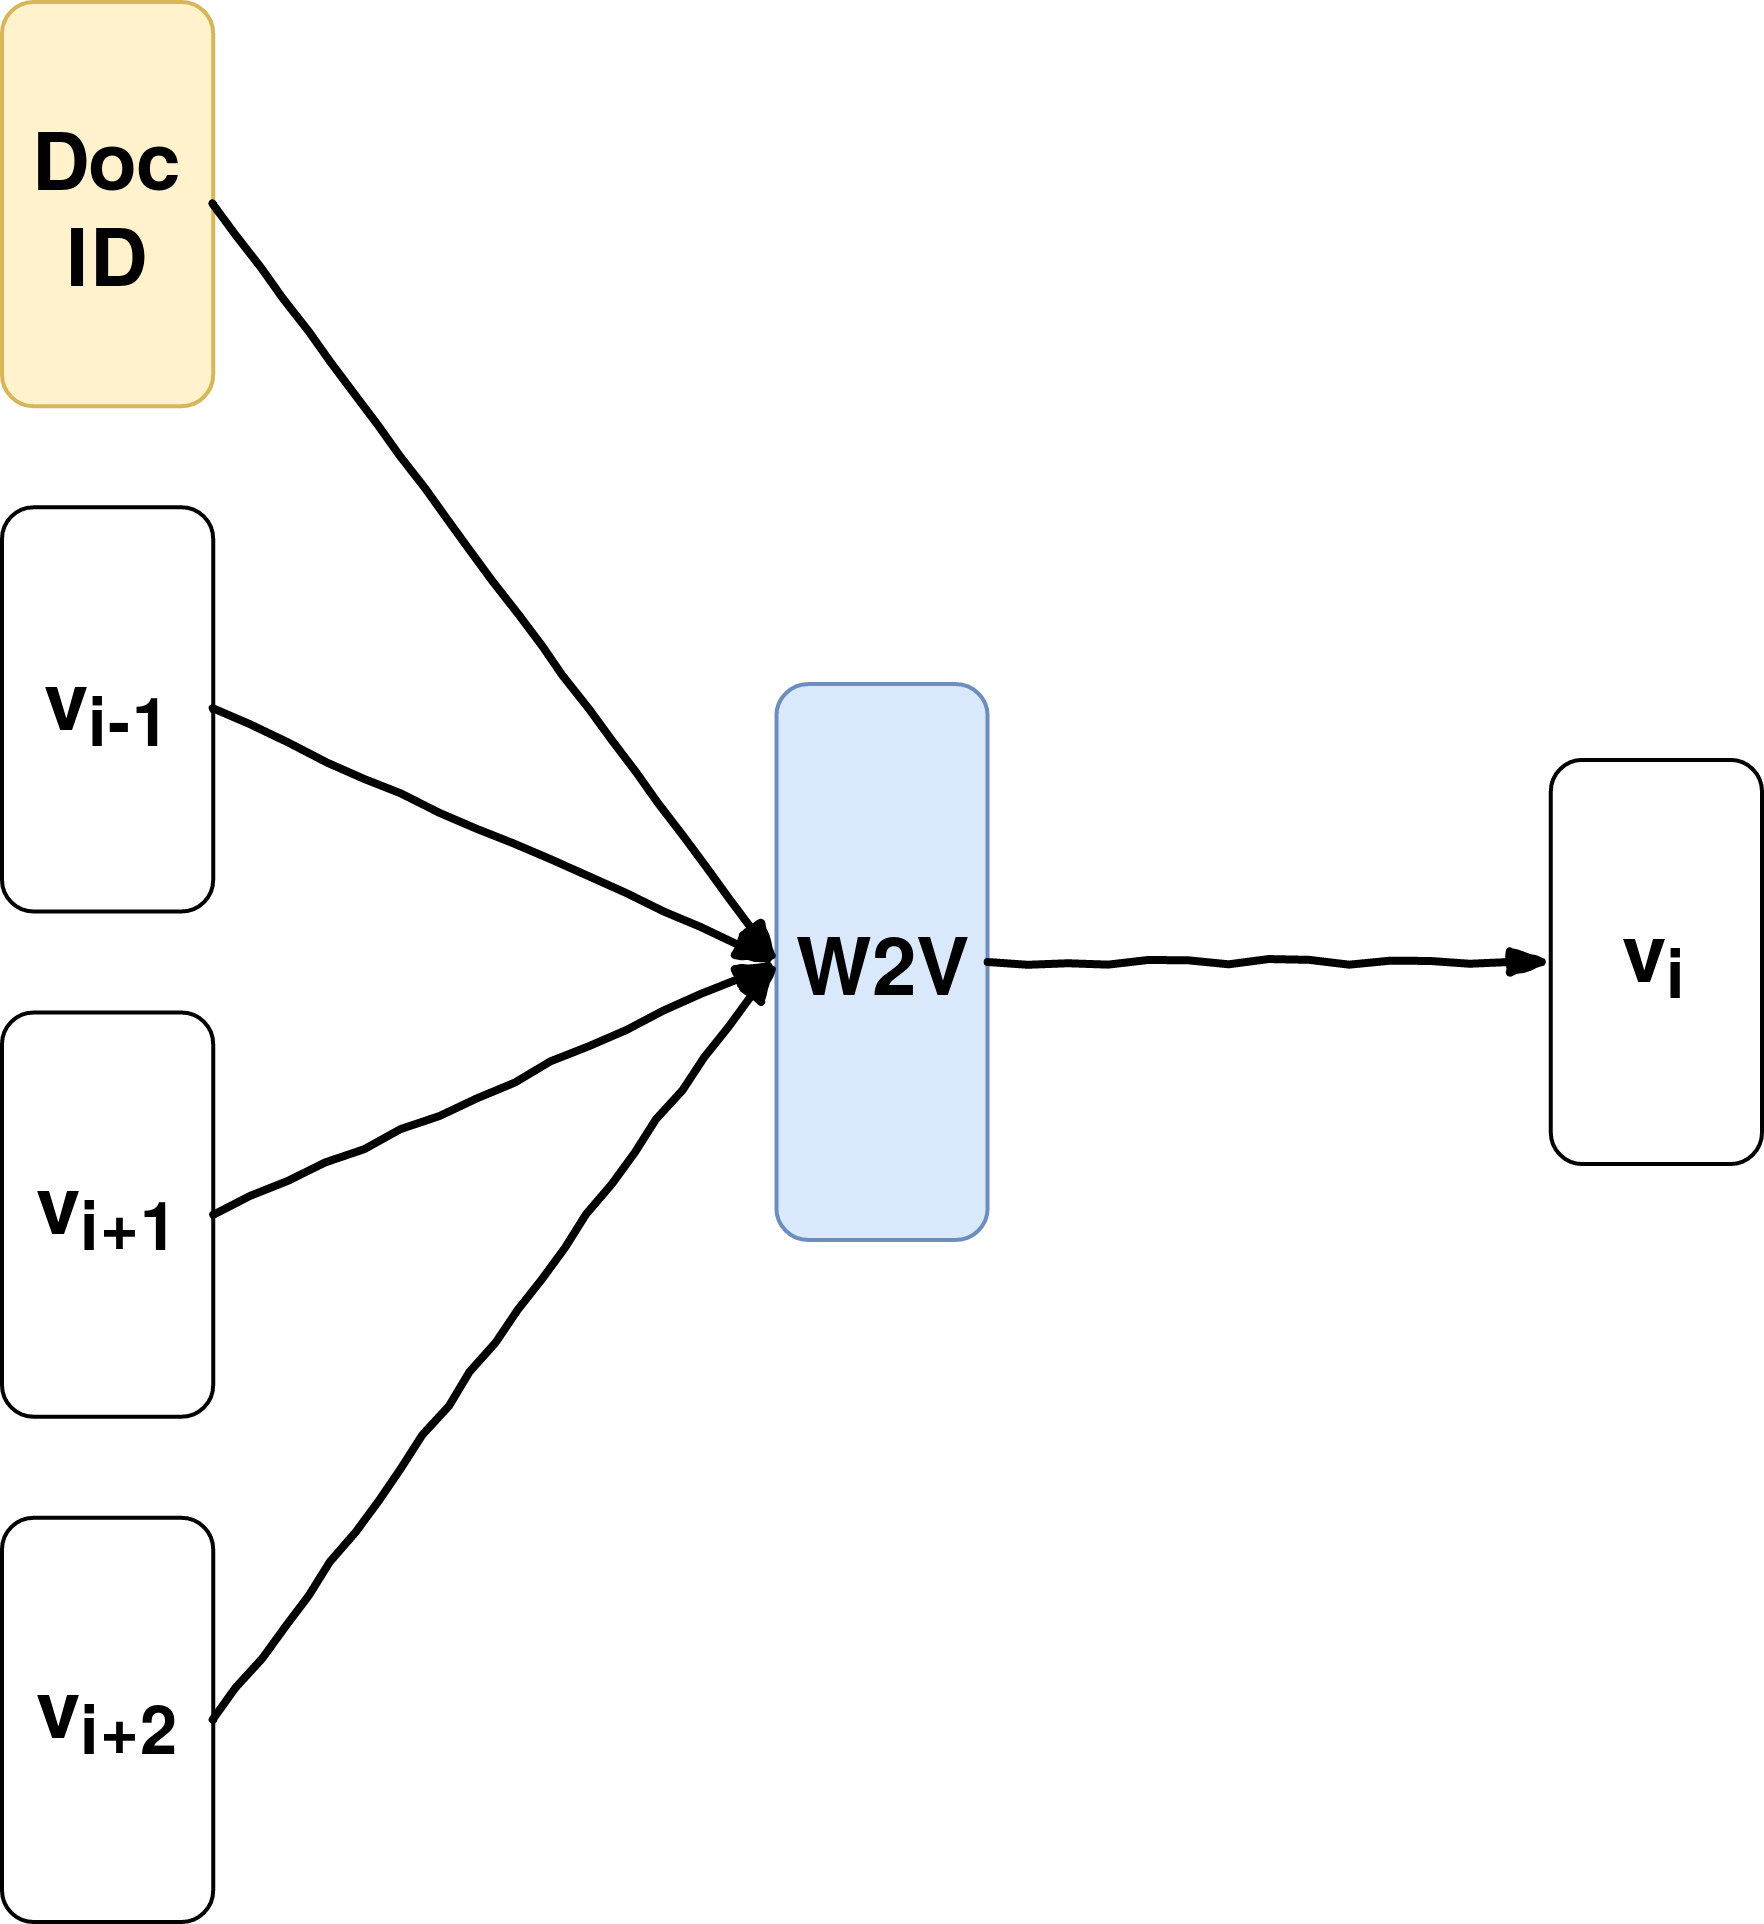
\includegraphics[width=0.5\textwidth,height=150px]{Doc2Vec}
	\caption{Doc2Vec PV-DM architektúra}
\end{figure}

A Word2Vec-hez hasonlóan a Doc2Vec-nek is létezik \textit{Skip-Gram} alternatívája, ez a PV-DBOW. A PV-DBOW modell gyorsabb és memóriahasználat szempontjából is gazdaságosabb a PV-DM-hez képest.

Mivel relatíve kevés algoritmus képes dokumentumszintű modellezésre és azok teljesítménye is limitált, a Doc2Vec egy jó választás lehet. A modell egyszerre mutat jó teljesítményt és a használata is könnyű.

\section{Transfer learning}

A modern szemantikus reprezentációs algoritmusok tanítása összetett folyamat. A feladatok során egyszerre kell több szempontra figyelni, melyek befolyásolhatják a modellünk pontosságát. Példának okáért mondatszintű reprezentációnknak képesnek kell lennie értelmezni a lexémák egymáshoz fűződő viszonyait és a mondatok közötti kohéziót is. A \textit{transfer learning} egy kiváló eszköz arra, hogy modellünket tanítsuk több aspektus szerint.

A \textit{transfer learning} napjainkban közkedvelt tanítási módszer, melynek ötletét az NLP ágazata a számítógépes látás eszközkészletéből merítette. A folyamatot két fázisra lehet bontani: előtanítás és a finomhangolás. Az előtanítás általában nagy mennyiségű adaton történik. A finomhangolás az előtanítás után kapott modell – adott NLP feladathoz szükséges – speciális feladatokon való tanítását jelenti, amely szignifikánsan kevesebb adatot igényel.

\begin{definition}
	Jelölje $D_s$ a forrástartományt, $D_t$ a céltartományt, $T_s$ a forrástartományhoz tartozó feladatot, továbbá $X_t$ és $Y_t$ rendre a $T_t$ célfeladathoz tartozó inputváltozók és  címkék halmazát. A \textbf{transfer learning} célja megtanulni $P(Y_t|X_t)$ feltételes eloszlást $D_t$-ben $D_s$ által gyűjtött információ alapján úgy, hogy $D_s \neq D_t$ vagy $T_s \neq T_t$.	 
\end{definition}

\begin{figure}[H]
	\centering
	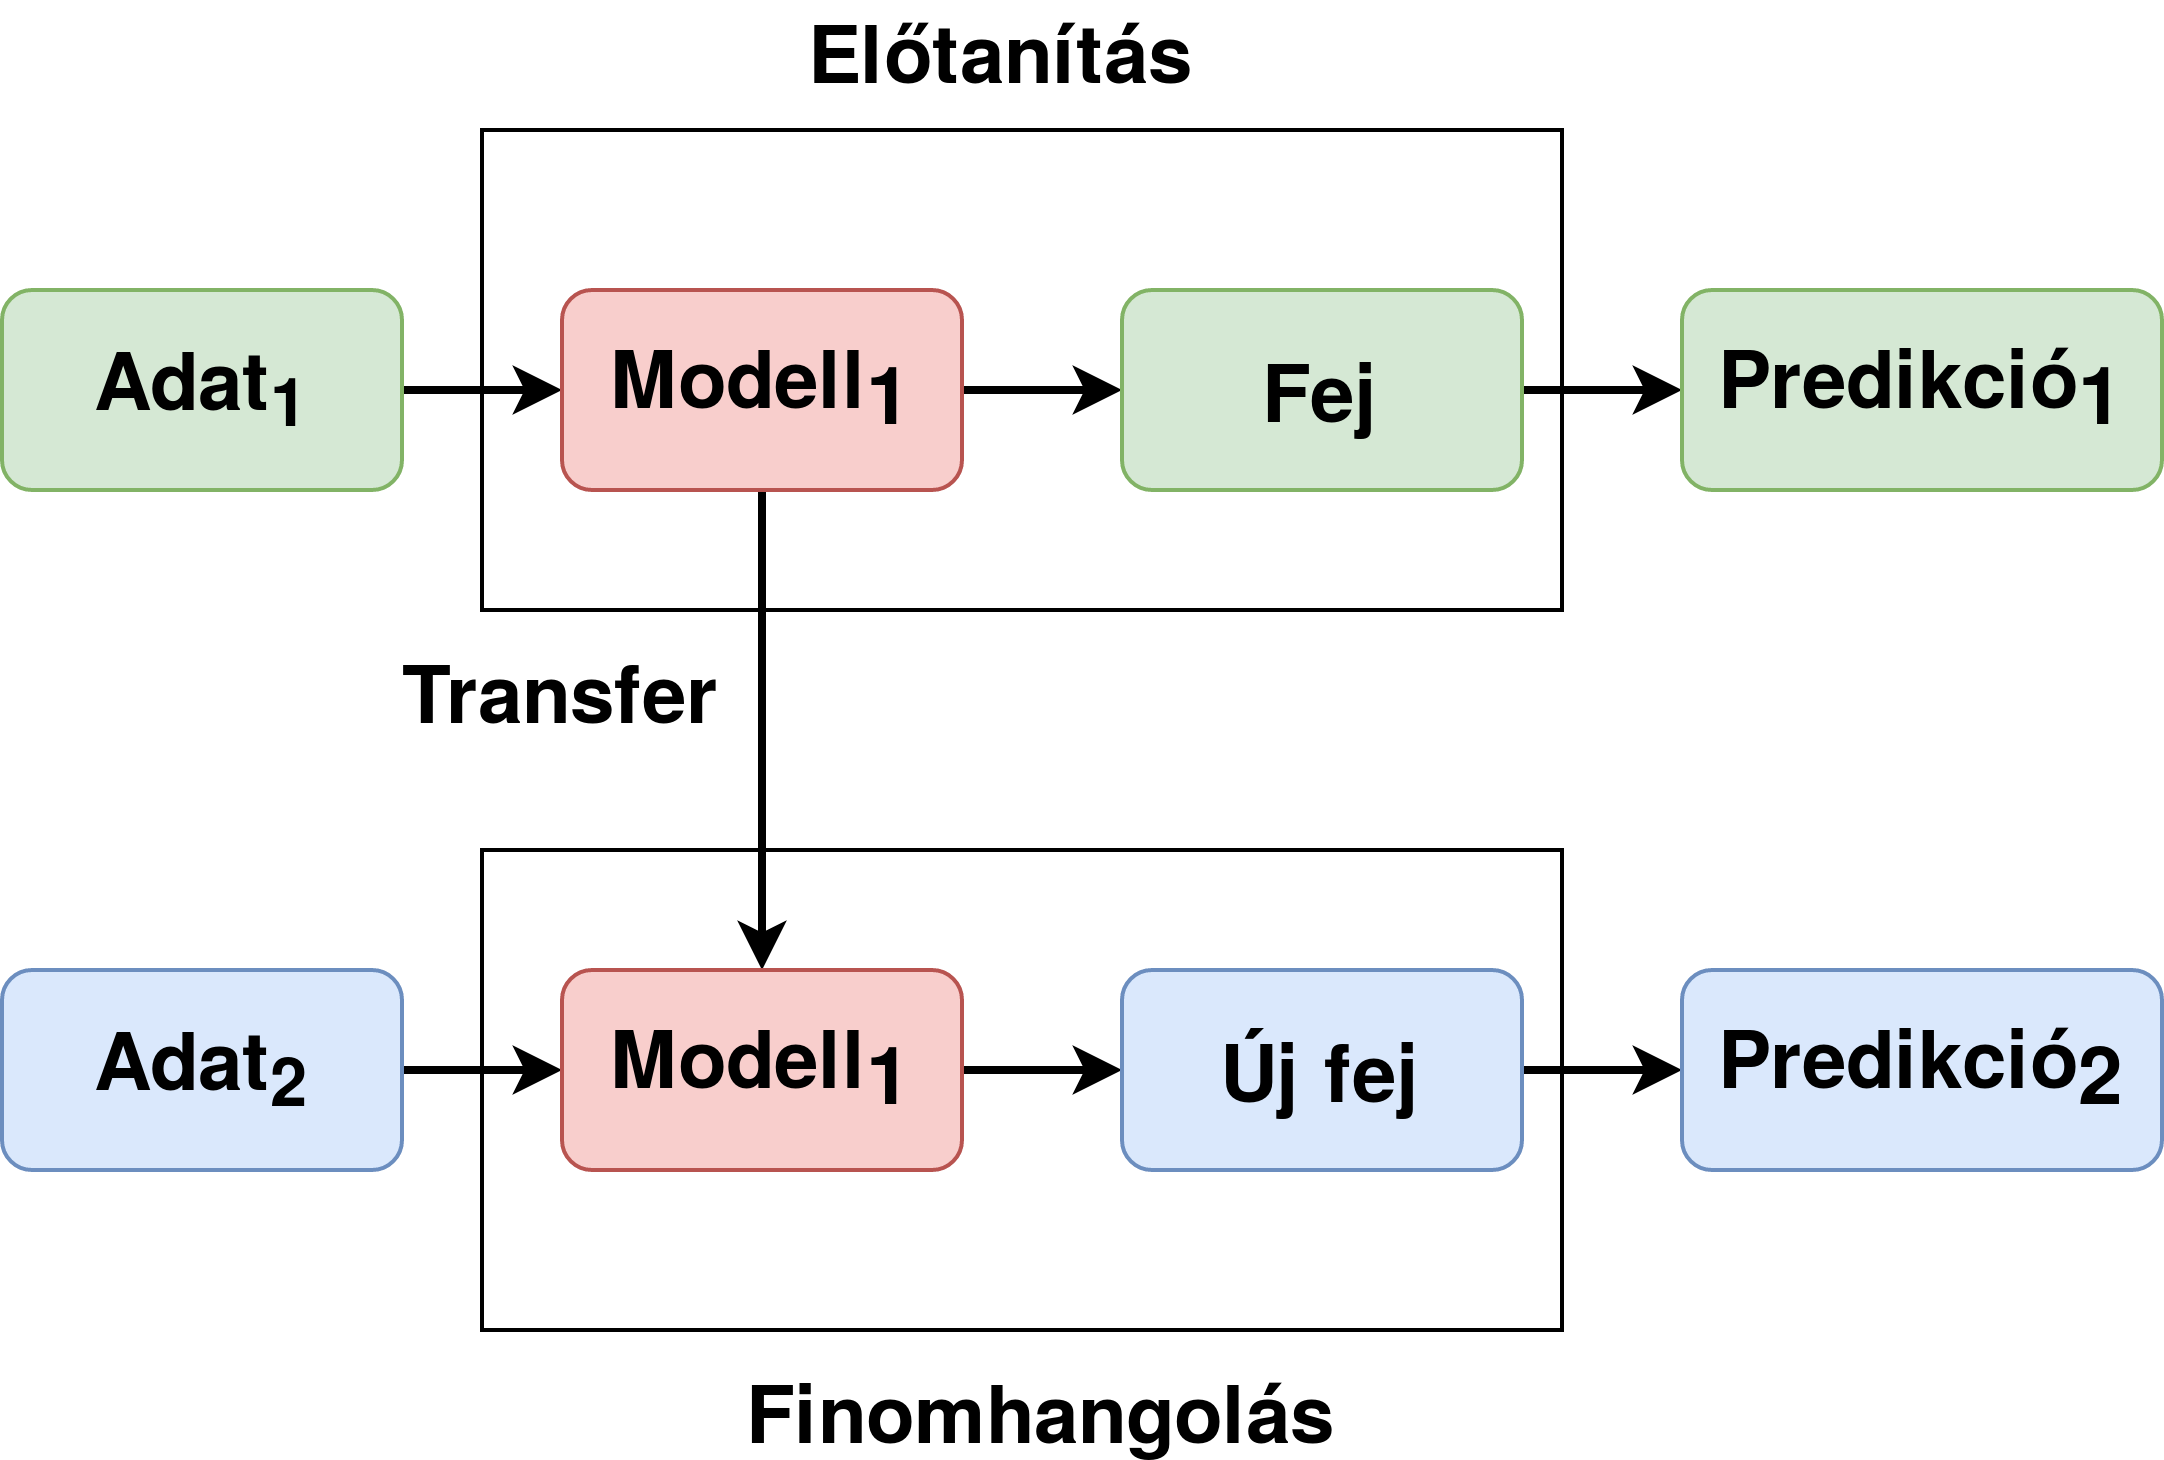
\includegraphics[width=0.6\textwidth,height=170px]{transfer}
	\caption{Transfer learning}
\end{figure}

Az előtanítási szakasz olyan feladattal kezdődik, mely kellőképpen generalizál és a neurális hálónk sok, hasznos és általános információhoz tud jutni. A folyamathoz használt adathalmaz általában nagy mennyiségű annotálatlan adatot tartalmaz, de vannak kivételek, például az InferSent esetében.

A finomhangolási fázis alatt használt feladatok az előtanítás után kapott modell súlyait alkalmazzák, de a bemeneti adatok és a feladatok végrehajtásához szükséges fej lehet eltérő is. Ezen szakasz állhat feladatok sorozatából is, ekkor a súlyokat inkrementálisan használják azok. A sikeres végrehajtást követően modellünk képes lesz komplexebb összefüggések felismerésére és pontosabb eredmény elérésére.

A jelenlegi trendek szerint a reprezentációs módszerek tanítási módja nagyobb hangsúlyt kap, mint maga a neurális háló szerkezete. A \textit{transfer learning} használata a numerikus ábrázolás során még kiaknázatlan terület, mely rendkívül sok eredményt hozhat a jövőben.








\cleardoublepage

\chapter{Felhasználói dokumentáció} % User guide
\label{ch:user}

Lorem ipsum dolor sit amet $\mathbb{N}$\nomenclature{$\mathbb{N}$}{Set of natural numbers}, consectetur adipiscing elit. Duis nibh leo, dapibus in elementum nec, aliquet id sem. Suspendisse potenti. Nullam sit amet consectetur nibh. Donec scelerisque varius turpis at tincidunt. Cras a diam in mauris viverra vehicula. Vivamus mi odio, fermentum vel arcu efficitur, lacinia viverra nibh. Aliquam aliquam ante mi, vel pretium arcu dapibus eu. Nulla finibus ante vel arcu tincidunt, ut consectetur ligula finibus. Mauris mollis lectus sed ipsum bibendum, ac ultrices erat dictum. Suspendisse faucibus euismod lacinia $\mathbb{Z}$\nomenclature{$\mathbb{Z}$}{Set of integer numbers}.


\section{Felsorolások} % Enumerations and lists

Etiam vel odio ante. Etiam pulvinar nibh quis massa auctor congue. Pellentesque quis odio vitae sapien molestie vestibulum sit amet et quam. Pellentesque vel dui eget enim hendrerit finibus at sit amet libero. Quisque sollicitudin ultrices enim, nec porta magna imperdiet vitae. Cras condimentum nunc dui, eget molestie nunc accumsan vel.

\begin{itemize}
	\item Fusce in aliquet neque, in pretium sem.
	\item Donec tincidunt tellus id lectus pretium fringilla.
	\item Nunc faucibus, erat pretium tempus tempor, tortor mi fringilla neque, ac congue ex dui vitae mauris.
\end{itemize}

Donec dapibus sodales ante, at scelerisque nunc laoreet sit amet. Mauris porttitor tincidunt neque, vel ullamcorper neque pulvinar et. Integer eu lorem euismod, faucibus lectus sed, accumsan felis. Nunc ornare mi at augue vulputate, eu venenatis magna mollis. Nunc sed posuere dui, et varius nulla. Sed mollis nibh augue, eget scelerisque eros ornare nec.

\begin{enumerate}
	\item\label{step:first} Donec pretium et quam a cursus. Ut sollicitudin tempus urna et mollis.
	\item Aliquam et aliquam turpis, sed fermentum mauris. Nulla eget ex diam.
	\item Donec eget tellus pharetra, semper neque eget, rutrum diam Step~\ref{step:first}.
\end{enumerate}

Praesent porta, metus eget eleifend consequat, eros ligula eleifend ex, a pellentesque mi est vitae urna. Vivamus turpis nunc, iaculis non leo eget, mattis vulputate tellus. Maecenas rutrum eros sem, pharetra interdum nulla porttitor sit amet. In vitae viverra ante. Maecenas sit amet placerat orci, sed tincidunt velit. Vivamus mattis, enim vel suscipit elementum, quam odio venenatis elit\footnote{Phasellus faucibus varius purus, nec tristique enim porta vitae.}, et mollis nulla nunc a risus. Praesent purus magna, tristique sed lacus sit amet, convallis malesuada magna. 

\begin{description}
	\item[Vestibulum venenatis] malesuada enim, ac auctor erat vestibulum et. Phasellus id purus a leo suscipit accumsan.
	\item[Orci varius natoque] penatibus et magnis dis parturient montes, nascetur ridiculus mus. Nullam interdum rhoncus nisl, vel pharetra arcu euismod sagittis. Vestibulum ac turpis auctor, viverra turpis at, tempus tellus.
	\item[Morbi dignissim] erat ut rutrum aliquet. Nulla eu rutrum urna. Integer non urna at mauris scelerisque rutrum sed non turpis.
\end{description}

\subsection{Szoros térközű felsorolások} % Lists with narrow spacing inbetween items

Phasellus ultricies, sapien sit amet ultricies placerat, velit purus viverra ligula, id consequat ipsum odio imperdiet enim:
\begin{compactenum}
	\item Maecenas eget lobortis leo.
	\item Donec eget libero enim.
	\item In eu eros a eros lacinia maximus ullamcorper eget augue.
\end{compactenum}

\bigskip

In quis turpis metus. Proin maximus nibh et massa eleifend, a feugiat augue porta. Sed eget est purus. Duis in placerat leo. Donec pharetra eros nec enim convallis:
\begin{compactitem}
	\item Pellentesque odio lacus.
	\item Maximus ut nisl auctor.
	\item Sagittis vulputate lorem.
\end{compactitem}

\bigskip

Vestibulum ante ipsum primis in faucibus orci luctus et ultrices posuere cubilia Curae; Sed lorem libero, dignissim vitae gravida a, ornare vitae est.
\begin{compactdesc}
	\item[Cras maximus] massa commodo pellentesque viverra.
	\item[Morbi sit] amet ante risus. Aliquam nec sollicitudin mauris
	\item[Ut aliquam rhoncus sapien] luctus viverra arcu iaculis posuere
\end{compactdesc}


\section{Képek, ábrák} % Images and figures

Aliquam vehicula luctus mi a pretium. Nulla quam neque, maximus nec velit in, aliquam mollis tortor. Aliquam erat volutpat. Curabitur vitae laoreet turpis. Integer id diam ligula. Nulla sodales purus id mi consequat, eu venenatis odio pharetra. Cras a arcu quam. Suspendisse augue risus, pulvinar a turpis et, commodo aliquet turpis. Nulla aliquam scelerisque mi eget pharetra. Mauris sed posuere elit, ac lobortis metus. Proin lacinia sit amet diam sed auctor. Nam viverra orci id sapien sollicitudin, a aliquam lacus suscipit, Figure~\ref{fig:example-1}:

\begin{figure}[H]
	\centering
	
\includegraphics[width=0.6\textwidth,height=100px]{elte_cimer_szines}
	\caption{Quisque ac tincidunt leo}
	\label{fig:example-1}
\end{figure}

\subsection{Képek szegélyezése} % Framing figures

Ut aliquet nec neque eget fermentum. Cras volutpat tellus sed placerat elementum. Quisque neque dui, consectetur nec finibus eget, blandit id purus. Nam eget ipsum non nunc placerat interdum.

\begin{figure}[H]
	\centering
	
\includegraphics[width=0.6\textwidth,height=100px,frame]{elte_cimer_szines}
	\caption{Quisque ac tincidunt leo}
\end{figure}

\subsection{Képek csoportosítása} % Subfigures

In non ipsum fermentum urna feugiat rutrum a at odio. Pellentesque habitant morbi tristique senectus et netus et malesuada fames ac turpis egestas. Nulla tincidunt mattis nisl id suscipit. Sed bibendum ac felis sed volutpat. Nam pharetra nisi nec facilisis faucibus. Aenean tristique nec libero non commodo. Nulla egestas laoreet tempus. Nunc eu aliquet nulla, quis vehicula dui. Proin ac risus sodales, gravida nisi vitae, efficitur neque, Figure~\ref{fig:example-2}:

\begin{figure}[H]
	\centering
	\subfigure[Vestibulum quis mattis urna]{
		
\includegraphics[width=0.45\linewidth]{elte_cimer_szines}}
	\hspace{5pt}
	\subfigure[Donec hendrerit quis dui sit amet venenatis]{
		
\includegraphics[width=0.45\linewidth]{elte_cimer_szines}}
	\caption{Aenean porttitor mi volutpat massa gravida}
	\label{fig:example-2}
\end{figure}

Nam et nunc eget elit tincidunt sollicitudin. Quisque ligula ipsum, tempor vitae tortor ut, commodo rhoncus diam. Pellentesque habitant morbi tristique senectus et netus et malesuada fames ac turpis egestas. Phasellus vehicula quam dui, eu convallis metus porta ac.


\section{Táblázatok} % Tables

Nam magna ex, euismod nec interdum sed, sagittis nec leo. Nam blandit massa bibendum mattis tristique. Phasellus tortor ligula, sodales a consectetur vitae, placerat vitae dolor. Aenean consequat in quam ac mollis. 

\begin{table}[H]
	\centering
	\begin{tabular}{ | m{0.25\textwidth} | m{0.65\textwidth} | }
		\hline
		\textbf{Phasellus tortor} & \textbf{Aenean consequat} \\
		\hline \hline
		\emph{Sed malesuada} & Aliquam aliquam velit in convallis ultrices. \\
		\hline
		\emph{Purus sagittis} &  Quisque lobortis eros vitae urna lacinia euismod. \\
		\hline
		\emph{Pellentesque} & Curabitur ac lacus pellentesque, eleifend sem ut, placerat enim. Ut auctor tempor odio ut dapibus. \\
		\hline
	\end{tabular}
	\caption{Maecenas tincidunt non justo quis accumsan}
	\label{tab:example-1}
\end{table}

\subsection{Sorok és oszlopok egyesítése} % Multi rows and multi columns

Mauris a dapibus lectus. Vestibulum commodo nibh ante, ut maximus magna eleifend vel. Integer vehicula elit non lacus lacinia, vitae porttitor dolor ultrices. Vivamus gravida faucibus efficitur. Ut non erat quis arcu vehicula lacinia. Nulla felis mauris, laoreet sed malesuada in, euismod et lacus. Aenean at finibus ipsum. Pellentesque dignissim elit sit amet lacus congue vulputate.

\begin{table}[htb]
	\centering
	\begin{tabular}{ | c | r | r | r | r | r | r | }
		\hline
		\multirow{2}{*}{\textbf{Quisque}} & \multicolumn{2}{ c | }{\textbf{Suspendisse}} & \multicolumn{2}{ c | }{\textbf{Aliquam}} & \multicolumn{2}{ c | }{\textbf{Vivamus}} \\
		\cline{2-7}
		& Proin & Nunc & Proin & Nunc & Proin & Nunc \\
		\hline \hline		
		Leo & 2,80 MB & 100\% & 232 KB & 8,09\% & 248 KB & 8,64\% \\
		\hline
		Vel & 9,60 MB & 100\% & 564 KB & 5,74\% & 292 KB & 2,97\% \\
		\hline
		Auge & 78,2 MB & 100\% & 52,3 MB & 66,88\% & 3,22 MB & 4,12\% \\
		\hline 
	\end{tabular}
	\caption[Rövid cím a táblázatjegyzékbe]{Vivamus ac arcu fringilla, fermentum neque sed, interdum erat. Mauris bibendum mauris vitae enim mollis, et eleifend turpis aliquet.}
	\label{tab:example-2}
\end{table}

\subsection{Több oldalra átnyúló táblázatok} % Long tables over multiple pages

Nunc porta placerat leo, sit amet porttitor dui porta molestie. Aliquam at fermentum mi. Maecenas vitae lorem at leo tincidunt volutpat at nec tortor. Vivamus semper lacus eu diam laoreet congue. Vivamus in ipsum risus. Nulla ullamcorper finibus mauris non aliquet. Vivamus elementum rhoncus ex ut porttitor.

\begin{center}
	\begin{longtable}{ | p{0.3\textwidth} | p{0.7\textwidth} | }
		
		\hline
		\multicolumn{2}{|c|}{\textbf{Praesent aliquam mauris enim}}
		\\ \hline
		
		\emph{Suspendisse potenti} & \emph{Lorem ipsum dolor sit amet}
		\\ \hline \hline
		\endfirsthead % első oldal fejléce
		
		\hline
		\emph{Suspendisse potenti} & \emph{Lorem ipsum dolor sit amet}
		\\ \hline \hline
		\endhead % többi oldal fejléce
		
		\hline
		\endfoot % többi oldal lábléce
		
		\endlastfoot % utolsó oldal lábléce
		
		\emph{Praesent}
		& Nulla ultrices et libero sit amet fringilla. Nunc scelerisque ante tempus sapien placerat convallis.
		\\ \hline
		
		\emph{Luctus}
		& Integer hendrerit erat massa, non hendrerit risus convallis at. Curabitur ultrices, justo in imperdiet condimentum, neque tortor luctus enim, luctus posuere massa erat vitae nibh.
		\\ \hline
		
		\emph{Egestas}
		& Duis fermentum feugiat augue in blandit. Mauris a tempor felis. Pellentesque ultricies tristique dignissim. Pellentesque aliquam semper tristique. Nam nec egestas dolor. Vestibulum id elit quis enim fringilla tempor eu a mauris. Aliquam vitae lacus tellus. Phasellus mauris lectus, aliquam id leo eget, auctor dapibus magna. Fusce lacinia felis ac elit luctus luctus.
		\\ \hline
		
		\emph{Dignissim}
		& Praesent aliquam mauris enim, vestibulum posuere massa facilisis in. Suspendisse potenti. Nam quam purus, rutrum eu augue ut, varius vehicula tellus. Fusce dui diam, aliquet sit amet eros at, sollicitudin facilisis quam. Phasellus tempor metus vel augue gravida pretium. Proin aliquam aliquam blandit. Nulla id tempus mi. Fusce in aliquam tortor.
		\\ \hline
		
		\emph{Pellentesque}
		& Donec felis nibh, imperdiet a arcu non, vehicula gravida nibh. Quisque interdum sapien eu massa commodo, ac elementum felis faucibus.
		\\ \hline
		
		\emph{Molestie}
		& Cras ullamcorper tellus et auctor ultricies. Maecenas tincidunt euismod lectus nec venenatis. Suspendisse potenti. Pellentesque pretium nunc ut euismod cursus. Nam venenatis condimentum quam. Curabitur suscipit efficitur aliquet. Interdum et malesuada fames ac ante ipsum primis in faucibus.
		\\ \hline
		
		\emph{Vivamus semper}
		& In purus purus, faucibus eu libero vulputate, tristique sodales nunc. Nulla ut gravida dolor. Fusce vel pellentesque mi, vel efficitur eros. Nunc vitae elit tellus. Sed vestibulum auctor consequat. 
		\\ \hline
		
		\emph{Condimentum}
		& Nulla scelerisque, leo et facilisis pretium, risus enim cursus turpis, eu suscipit ipsum ipsum in mauris. Praesent eget pulvinar ipsum, suscipit interdum nunc. Nam varius massa ut justo ullamcorper sollicitudin. Vivamus facilisis suscipit neque, eu fermentum risus. Ut at mi mauris.
		\\ \hline
		
		\caption{Praesent ullamcorper consequat tellus ut eleifend}
		\label{tab:example-3}		
	\end{longtable}
\end{center}
\cleardoublepage

\chapter{Fejlesztői dokumentáció} % Developer guide
\label{ch:impl}

Lorem ipsum dolor sit amet, consectetur adipiscing elit. Duis nibh leo, dapibus in elementum nec, aliquet id sem. Suspendisse potenti. Nullam sit amet consectetur nibh. Donec scelerisque varius turpis at tincidunt.


\section{Tételek, definíciók, megjegyzések} % Theorem-like items

\begin{definition}
Mauris tristique sollicitudin ultrices. Etiam tristique quam sit amet metus dictum imperdiet. Nunc id lorem sed nisl pulvinar aliquet vitae quis arcu. Morbi iaculis eleifend porttitor.
\end{definition}

Maecenas rutrum eros sem, pharetra interdum nulla porttitor sit amet. In vitae viverra ante. Maecenas sit amet placerat orci, sed tincidunt velit. Vivamus mattis, enim vel suscipit elementum, quam odio venenatis elit, et mollis nulla nunc a risus. Praesent purus magna, tristique sed lacus sit amet, convallis malesuada magna. Phasellus faucibus varius purus, nec tristique enim porta vitae.

\begin{theorem}
Nulla finibus ante vel arcu tincidunt, ut consectetur ligula finibus. Mauris mollis lectus sed ipsum bibendum, ac ultrices erat dictum. Suspendisse faucibus euismod lacinia. Etiam vel odio ante.
\end{theorem}
\begin{proof}
Etiam pulvinar nibh quis massa auctor congue. Pellentesque quis odio vitae sapien molestie vestibulum sit amet et quam. Pellentesque vel dui eget enim hendrerit finibus at sit amet libero. Quisque sollicitudin ultrices enim, nec porta magna imperdiet vitae. Cras condimentum nunc dui.
\end{proof}

Donec dapibus sodales ante, at scelerisque nunc laoreet sit amet. Mauris porttitor tincidunt neque, vel ullamcorper neque pulvinar et. Integer eu lorem euismod, faucibus lectus sed, accumsan felis. 

\begin{remark}
Nunc ornare mi at augue vulputate, eu venenatis magna mollis. Nunc sed posuere dui, et varius nulla. Sed mollis nibh augue, eget scelerisque eros ornare nec. Praesent porta, metus eget eleifend consequat, eros ligula eleifend ex, a pellentesque mi est vitae urna. Vivamus turpis nunc, iaculis non leo eget, mattis vulputate tellus.
\end{remark}

Fusce in aliquet neque, in pretium sem. Donec tincidunt tellus id lectus pretium fringilla. Nunc faucibus, erat pretium tempus tempor, tortor mi fringilla neque, ac congue ex dui vitae mauris. Donec pretium et quam a cursus.

\begin{note}
Aliquam vehicula luctus mi a pretium. Nulla quam neque, maximus nec velit in, aliquam mollis tortor. Aliquam erat volutpat. Curabitur vitae laoreet turpis. Integer id diam ligula.
\end{note}

Ut sollicitudin tempus urna et mollis. Aliquam et aliquam turpis, sed fermentum mauris. Nulla eget ex diam. Donec eget tellus pharetra, semper neque eget, rutrum diam.

\subsection{Egyenletek, matematika} % Equations, formulas

Duis suscipit ipsum nec urna blandit, $2 + 2 = 4$ pellentesque vehicula quam fringilla. Vivamus euismod, lectus sit amet euismod viverra, dolor metus consequat sapien, ut hendrerit nisl nulla id nisi. Nam in leo eu quam sollicitudin semper a quis velit.

$$a^2 + b^2 = c^2$$

Phasellus mollis, elit sed convallis feugiat, dolor quam dapibus nibh, suscipit consectetur lacus risus quis sem. Vivamus scelerisque porta odio, vitae euismod dolor accumsan ut.

In mathematica, identitatem Euleri (equation est scriptor vti etiam notum) sit aequalitatem Equation~\ref{eq:euler}:
\begin{equation}\label{eq:euler}
e^{i \times \pi} + 1 = 0
\end{equation}


\section{Forráskódok} % Source code samples

Nulla sodales purus id mi consequat, eu venenatis odio pharetra. Cras a arcu quam. Suspendisse augue risus, pulvinar a turpis et, commodo aliquet turpis. Nulla aliquam scelerisque mi eget pharetra. Mauris sed posuere elit, ac lobortis metus. Proin lacinia sit amet diam sed auctor. Nam viverra orci id sapien sollicitudin, a aliquam lacus suscipit. Quisque ac tincidunt leo Code~\ref{src:cpp} and \ref{src:csharp}:

\lstset{caption={Hello World in C++}, label=src:cpp}
\begin{lstlisting}[language={C++}]
#include <stdio>

int main() 
{
	int c;
	std::cout << "Hello World!" << std::endl;

	std::cout << "Press any key to exit." << std::endl;
	std::cin >> c;
	
	return 0;
}
\end{lstlisting}

\lstset{caption={Hello World in C\#}, label=src:csharp}
\begin{lstlisting}[language={[Sharp]C}]
using System;
namespace HelloWorld
{
	class Hello 
	{
		static void Main() 
		{
			Console.WriteLine("Hello World!");
			
			Console.WriteLine("Press any key to exit.");
			Console.ReadKey();
		}
	}
}
\end{lstlisting}

\subsection{Algoritmusok} % Algorithms

A general Interval Branch and Bound algorithm is shown in Algorithm~\ref{alg:ibb}. One of the following selection rules is applied in Step \ref{step:selrule}.\\
Példa forrása: \href{https://www.inf.u-szeged.hu/actacybernetica/}{Acta Cybernetica (ez egy link)}.

\begin{algorithm}[H]
\caption{A general interval B\&B algorithm} 
\label{alg:ibb} 
\textbf{\underline{Funct}} IBB($S,f$)
\begin{algorithmic}[1] % sorszámok megjelenítése minden n. sor előtt, most n = 1
\STATE Set the working list ${\cal L}_W$ := $\{S\}$ and the final list ${\cal L}_Q$ := $\{\}$     
\WHILE{( ${\cal L}_W \neq \emptyset$ )} \label{alg:igoend}
	\STATE  Select an interval $X$ from ${\cal L}_W$ \label{step:selrule}\COMMENT{Selection rule}  
	\STATE Compute $lbf(X)$ \COMMENT{Bounding rule}		  
	\IF[Elimination rule]{$X$ cannot be eliminated}
		\STATE Divide $X$ into $X^j,\ j=1,\dots, p$, subintervals   \COMMENT{Division rule}
		\FOR{$j=1,\ldots,p$}
			\IF[Termination rule]{$X^j$ satisfies the termination criterion}
				\STATE Store $X^j$ in ${\cal L}_W$ 
			\ELSE
				\STATE Store $X^j$ in ${\cal L}_W$ 
			\ENDIF
		\ENDFOR  
	\ENDIF
\ENDWHILE
\STATE \textbf{return} ${\cal L}_Q$
\end{algorithmic}
\end{algorithm}

\cleardoublepage

\chapter{Összegzés} % Conclusion
\label{ch:sum}

A természetes szövegfeldolgozás és annak ágazata, a szemantikus reprezentációk mind akadémiai, mind ipari értelemben gyorsuló ütemben fejlődő területek, amelyek a mai napig rengeteg felderítésre váró lehetőséget tartogatnak. A numerikus ábrázoló algoritmusok teljesítményének növekedése olyan gyakorlati alkalmazások pontosságának javulását indukálják, melyek segítségével hatékonyan kiszűrhető a gyűlöletbeszéd a szociális médiából, vagy akár eredményesen felvehető a harc az álhírek terjedésével szemben. 

Diplomamunkám végeredménye egy kétirányú mondat- és paragrafusszintű előre tanított szemantikus reprezentációs modell, amely képes leképezni a magyar nyelven írt mondatokat a szemantikus térbe.

Magyar nyelvű tanítóadat a nyelv beszéltségéből fakadóan nem, vagy csak elvétve elérhető. A módszer tanításához használt adathalmaz előállítása nem igényel emberi címkézést, olcsó és a végtelenségig skálázható. Továbbá a tanításra szolgáló feladatok jellegéből fakadóan, az algoritmus jó eséllyel átültethető más kis és közepes nyelvre is.

A munkám során több, különféle magyar nyelvű adathalmazt vizsgáltam, melyek akár Word2Vec modellek, akár a bemutatott nyelvi modell létrehozására is alkalmasak lehetnek. Majd konstruáltam egy olyan, a magyar nyelvű szemantikus reprezentációs algoritmusok teljesítményének összehasonlítására használható halmazt, amelyen bináris klasszifikáció végezhető az elemek érzelmi tartalma alapján.
 
A dolgozatban bemutatott modellek tanítása során számos paraméterrel és beállítással próbálkoztam, majd ezek közül a legjobban teljesítő jelöltek teljesítményét a prezentált adathalmaz segítségével kimértem és összehasonlító elemzéseket végeztem.

%TODO: EREDMÉNYEK
interpretálás



\section{Javítási lehetőségek}
A szemantikus reprezentációs módszerekben rejlő lehetőségek a mai napig ismeretlenek és feltérképezetlenek. A tanulás vagy vektorgenerálás során optimalizált paraméterbeállítások és kombinációk további teljesítménybeli javulást hozhatnak.

A jövőben érdemes lehet az SGD helyett más optimalizáló algoritmust választani, továbbá a mélyhálóban alkalmazott \textit{max pooling}-ot \textit{mean pooling}-ra cserélni.

A megfigyelések alapján a GloVe szóbeágyazási módszer jobb eredményeket ér el, mint a Word2Vec, így célravezető lehet a beágyazási rétegben GloVe-ot használni.

Bizonyos esetekben a mélyebb architektúrák hatékonyabban tudják kinyerni a szekvenciális szöveges adatokból származó információkat, így több egymásra illesztett BiLSTM, vagy akár BiGRU réteg együttes tanítása pontosabb végeredményhez vezethet.

Az általam létrehozott nyelvi modellek mindegyike előtanított, finomhangolást nem végeztem rajtuk. A \textit{transfer learning} segítségével finomhangolt modellek több esetben jelentősen jobban teljesítenek, továbbá adatigényük is kisebb az előtanításénál. A jövőben a meglévő neurális modelleket egy olyan feladattal tervezem tovább tanítani, amelyben a háló célja egy értelmező kéziszótárból kinyert cikkek alapján kitalálni a cikkekhez tartozó szót.

Jelen működés szerint a maszkolt szavak közül csak a \textit{padding} token-ek kerülnek 0 súllyal a bemenetre. Ha sok ismeretlen szó található a tanítási halmazban, akkor a modellünk elfogulttá válhat az ismeretlen szavakat reprezentáló token felé, így nehezebbé téve a tanulási folyamatot. Ennélfogva előfordulhat, hogy az ilyen token-ek nullával való súlyozása jobb konvergációra készteti a modellt.

\chapter*{Összegzés - folytatás}

\section{Köszönetnyilvánítás}

magyar NLP ezen ágát egy kicsit katalizálja; az előtanítási módszereket és a benchmarkot is fel tudják használni és tovább tanítani

köszönet
\cleardoublepage

% Függelékek (opcionális) - hosszabb részletező táblázatok, sok és/vagy nagy kép esetén hasznos
% Appendices (optional) - useful for detailed information in long tables, many and/or large figures, etc.
\appendix
\chapter{Szimulációs eredmények} % Simulation results
\label{appx:simulation}

Lorem ipsum dolor sit amet, consectetur adipiscing elit. Pellentesque facilisis in nibh auctor molestie. Donec porta tortor mauris. Cras in lacus in purus ultricies blandit. Proin dolor erat, pulvinar posuere orci ac, eleifend ultrices libero. Donec elementum et elit a ullamcorper. Nunc tincidunt, lorem et consectetur tincidunt, ante sapien scelerisque neque, eu bibendum felis augue non est. Maecenas nibh arcu, ultrices et libero id, egestas tempus mauris. Etiam iaculis dui nec augue venenatis, fermentum posuere justo congue. Nullam sit amet porttitor sem, at porttitor augue. Proin bibendum justo at ornare efficitur. Donec tempor turpis ligula, vitae viverra felis finibus eu. Curabitur sed libero ac urna condimentum gravida. Donec tincidunt neque sit amet neque luctus auctor vel eget tortor. Integer dignissim, urna ut lobortis volutpat, justo nunc convallis diam, sit amet vulputate erat eros eu velit. Mauris porttitor dictum ante, commodo facilisis ex suscipit sed.

Sed egestas dapibus nisl, vitae fringilla justo. Donec eget condimentum lectus, molestie mattis nunc. Nulla ac faucibus dui. Nullam a congue erat. Ut accumsan sed sapien quis porttitor. Ut pellentesque, est ac posuere pulvinar, tortor mauris fermentum nulla, sit amet fringilla sapien sapien quis velit. Integer accumsan placerat lorem, eu aliquam urna consectetur eget. In ligula orci, dignissim sed consequat ac, porta at metus. Phasellus ipsum tellus, molestie ut lacus tempus, rutrum convallis elit. Suspendisse arcu orci, luctus vitae ultricies quis, bibendum sed elit. Vivamus at sem maximus leo placerat gravida semper vel mi. Etiam hendrerit sed massa ut lacinia. Morbi varius libero odio, sit amet auctor nunc interdum sit amet.

Aenean non mauris accumsan, rutrum nisi non, porttitor enim. Maecenas vel tortor ex. Proin vulputate tellus luctus egestas fermentum. In nec lobortis risus, sit amet tincidunt purus. Nam id turpis venenatis, vehicula nisl sed, ultricies nibh. Suspendisse in libero nec nisi tempor vestibulum. Integer eu dui congue enim venenatis lobortis. Donec sed elementum nunc. Nulla facilisi. Maecenas cursus id lorem et finibus. Sed fermentum molestie erat, nec tempor lorem facilisis cursus. In vel nulla id orci fringilla facilisis. Cras non bibendum odio, ac vestibulum ex. Donec turpis urna, tincidunt ut mi eu, finibus facilisis lorem. Praesent posuere nisl nec dui accumsan, sed interdum odio malesuada.
\cleardoublepage

% Irodalomjegyzék (kötelező)
% Bibliography (mandatory)
\addcontentsline{toc}{chapter}{\biblabel}
\printbibliography[title=\biblabel]
\cleardoublepage

% Ábrajegyzék (opcionális) - 3-5 ábra fölött érdemes
% List of figures (optional) - useful over 3-5 figures
\addcontentsline{toc}{chapter}{\lstfigurelabel}
\listoffigures
\cleardoublepage

% Táblázatjegyzék (opcionális) - 3-5 táblázat fölött érdemes
% List of tables (optional) - useful over 3-5 tables
\addcontentsline{toc}{chapter}{\lsttablelabel}
\listoftables
\cleardoublepage

% Forráskódjegyzék (opcionális) - 3-5 kódpélda fölött érdemes
% List of codes (optional) - useful over 3-5 code samples
\addcontentsline{toc}{chapter}{\lstcodelabel}
\lstlistoflistings
\cleardoublepage

% Jelölésjegyzék (opcionális)
% List of symbols (optional)
%\printnomenclature

\end{document}
